\documentclass[letter]{article}

%% Language and font encodings
\usepackage[english]{babel}
\usepackage[utf8x]{inputenc}
\usepackage[T1]{fontenc}
\usepackage{enumitem}
\usepackage{fancyhdr}
\usepackage{tikz}
%% Useful packages
\usepackage{amsmath,amssymb}
\usepackage{graphicx}
\usepackage{cancel}
\usetikzlibrary{arrows.meta, decorations.pathreplacing, calc, angles, quotes}
\usepackage{pgfplots}
\pgfplotsset{compat=newest}
\usepackage[
  colorlinks       = true,
  linkcolor        = blue,
  urlcolor         = cyan,
  citecolor        = green,
]{hyperref}

\setlength{\headheight}{14pt}
\setlength{\parindent}{0pt}
\setlength{\parskip}{0.6em}
\setcounter{tocdepth}{2}

\pagestyle{fancy}
\lhead{MAT040 Beginning Algebra}
\renewcommand{\sectionmark}[1]{\markright{#1}}
\renewcommand{\subsectionmark}[1]{}
\rhead{\rightmark}
\cfoot{}
\rfoot{\thepage}

%% ---------- Shared macros ----------
\newsavebox{\keyboxsave}
\newenvironment{keybox}
  {\begin{lrbox}{\keyboxsave}\begin{minipage}{\dimexpr\linewidth-2\fboxsep-2\fboxrule\relax}}
  {\end{minipage}\end{lrbox}\par\noindent\fbox{\usebox{\keyboxsave}}\par}
\newcommand{\exbox}[1]{\fbox{\textbf{Example #1}}}
% Each chapter sets \chp, so example labels are unique across the whole book
\newcommand{\chp}{}
\newcommand{\solsec}[1]{\phantomsection\label{sec:\chp ex#1}\subsubsection*{Example #1}}
\newcommand{\seesol}[1]{See \hyperref[sec:\chp ex#1]{Example #1 in the solutions}.}
\newcommand{\chk}{\ \checkmark}
\newcommand{\source}[1]{\lfoot{\scriptsize Adapted from OpenStax \textit{#1}, CC BY 4.0}}

% Fraction pictures: \fracgrid{rows}{cols}{shaded}, \fracpie{slices}{shaded}
\newcommand{\fracgrid}[3]{%
\begin{tikzpicture}[baseline=0pt]
  \pgfmathtruncatemacro{\lastcell}{#1*#2-1}
  \foreach \i in {0,...,\lastcell}{
    \pgfmathtruncatemacro{\cx}{mod(\i,#2)}
    \pgfmathtruncatemacro{\cy}{int(\i/#2)}
    \ifnum\i<#3 \fill[gray!45] ({0.6*\cx},{-0.6*\cy-0.6}) rectangle ++(0.6,0.6);\fi
  }
  \draw[step=0.6] (0,{-0.6*#1}) grid ({0.6*#2},0);
\end{tikzpicture}}
\newcommand{\fracpie}[2]{%
\begin{tikzpicture}[baseline=0pt]
  \pgfmathtruncatemacro{\lastslice}{#1-1}
  \foreach \i in {0,...,\lastslice}{
    \pgfmathsetmacro{\a}{90-360/#1*\i}
    \pgfmathsetmacro{\b}{90-360/#1*(\i+1)}
    \ifnum\i<#2 \fill[gray!45] (0,0) -- (\a:0.9) arc (\a:\b:0.9) -- cycle;\fi
    \draw (0,0) -- (\a:0.9);
  }
  \draw (0,0) circle (0.9);
\end{tikzpicture}}
% Factor tree: \ftree{number}{prime/rest, prime/rest, ...}{number of steps}
\newcommand{\ftree}[3]{%
\begin{tikzpicture}[x=0.55cm,y=-0.75cm,every node/.style={inner sep=2pt}]
  \node (n0) at (0,0) {$#1$};
  \foreach \p/\r [count=\i from 1] in {#2}{
    \pgfmathtruncatemacro{\prev}{\i-1}
    \pgfmathtruncatemacro{\px}{\i-2}
    \node[circle,draw] (p\i) at (\px,\i) {$\p$};
    \node (n\i) at (\i,\i) {$\r$};
    \draw (n\prev.south) -- (p\i.north);
    \draw (n\prev.south) -- (n\i.north);
  }
  \node[circle,draw,inner sep=2pt] at (n#3) {$\phantom{0}$};
\end{tikzpicture}}

% A coordinate plane, -6..6 by -8..8, same as the grids on the worksheets
\pgfplotsset{
  plane/.style={
    width=0.48\textwidth, height=0.6\textwidth,
    xmin=-6, xmax=6, ymin=-8, ymax=8,
    axis lines=middle, grid=both,
    xtick={-6,-4,...,6}, ytick={-8,-6,...,8},
    minor xtick={-6,-5,...,6}, minor ytick={-8,-7,...,8},
    grid style={line width=.1pt, draw=gray!50},
    tick label style={font=\tiny},
    xlabel={$x$}, ylabel={$y$},
    every axis x label/.style={at={(ticklabel* cs:1.0)},anchor=west},
    every axis y label/.style={at={(ticklabel* cs:1.0)},anchor=south},
    title style={font=\small},
  },
  smallplane/.style={
    plane, width=0.6\textwidth, height=0.6\textwidth,
    xmin=-5, xmax=5, ymin=-5, ymax=5,
    xtick={-4,-2,...,4}, ytick={-4,-2,...,4},
    minor xtick={-5,-4,...,5}, minor ytick={-5,-4,...,5},
    enlargelimits=false,
  },
}

% Inequality number line: \ineqline{lo}{hi}{point}{type}{label}
% type: 1 = x>a, 2 = x>=a, 3 = x<a, 4 = x<=a, 5 = all reals, 6 = no solution
\newcommand{\ineqline}[5]{%
\pgfmathsetmacro{\xs}{7/(#2-#1)}%
\begin{tikzpicture}[x={\xs cm},>=Stealth]
  \draw[<->] (#1-0.4,0) -- (#2+0.4,0);
  \foreach \i in {#1,...,#2}{\draw (\i,0.1) -- (\i,-0.1) node[below=4pt,font=\small] {$\i$};}
  \coordinate (P) at (#3,0);
  \ifcase#4\or
    \draw[ultra thick,blue!60,->] (P) -- (#2+0.4,0);
    \draw[thick] ([xshift=1mm,yshift=2.2mm]P) .. controls ([xshift=-1mm,yshift=1mm]P) and ([xshift=-1mm,yshift=-1mm]P) .. ([xshift=1mm,yshift=-2.2mm]P);
  \or
    \draw[ultra thick,blue!60,->] (P) -- (#2+0.4,0);
    \draw[thick] ([xshift=1.5mm,yshift=2.2mm]P) -- ([yshift=2.2mm]P) -- ([yshift=-2.2mm]P) -- ([xshift=1.5mm,yshift=-2.2mm]P);
  \or
    \draw[ultra thick,blue!80!black,->] (P) -- (#1-0.4,0);
    \draw[thick] ([xshift=-1mm,yshift=2.2mm]P) .. controls ([xshift=1mm,yshift=1mm]P) and ([xshift=1mm,yshift=-1mm]P) .. ([xshift=-1mm,yshift=-2.2mm]P);
  \or
    \draw[ultra thick,blue!80!black,->] (P) -- (#1-0.4,0);
    \draw[thick] ([xshift=-1.5mm,yshift=2.2mm]P) -- ([yshift=2.2mm]P) -- ([yshift=-2.2mm]P) -- ([xshift=-1.5mm,yshift=-2.2mm]P);
  \or
    \draw[ultra thick,blue!60,<->] (#1-0.4,0) -- (#2+0.4,0);
  \or
  \fi
  \ifx\relax#5\relax\else\node[above=3.5mm,font=\small] at (P) {$#5$};\fi
\end{tikzpicture}}

% Geoboard: \geoboard{drawing commands in peg coordinates 0..4}
\newcommand{\geoboard}[1]{%
\begin{tikzpicture}[scale=0.5]
  \fill[blue!8] (-0.6,-0.6) rectangle (4.6,4.6);
  \draw[blue!40] (-0.6,-0.6) rectangle (4.6,4.6);
  \foreach \gx in {0,...,4}{\foreach \gy in {0,...,4}{\fill[gray] (\gx,\gy) circle (0.07);}}
  #1
\end{tikzpicture}}

% Coordinate plane style
\pgfplotsset{
  gp/.style={
    width=0.46\textwidth, height=0.46\textwidth,
    axis lines=middle, grid=both, axis on top,
    grid style={line width=.1pt, draw=gray!45},
    xmin=-6, xmax=6, ymin=-6, ymax=6,
    xtick={-6,-4,...,6}, ytick={-6,-4,...,6},
    minor xtick={-6,-5,...,6}, minor ytick={-6,-5,...,6},
    tick label style={font=\tiny},
    xlabel={$x$}, ylabel={$y$},
    every axis x label/.style={at={(ticklabel* cs:1.0)},anchor=west},
    every axis y label/.style={at={(ticklabel* cs:1.0)},anchor=south},
    title style={font=\small},
  },
}

% Line with rise/run triangle: \slopefig{axis options}{x1}{y1}{x2}{y2}{function}{domain min}{domain max}
\newcommand{\slopefig}[8]{%
\begin{tikzpicture}\begin{axis}[gp,#1]
  \addplot[thick,blue,<->,domain=#7:#8,samples=2]{#6};
  \draw[red,thick] (axis cs:#2,#3) -- (axis cs:#4,#3) -- (axis cs:#4,#5);
  \addplot[only marks,mark=*,blue] coordinates {(#2,#3)(#4,#5)};
  \node[red,font=\scriptsize,above] at (axis cs:{(#2+#4)/2},#3) {run};
  \node[red,font=\scriptsize,right] at (axis cs:#4,{(#3+#5)/2}) {rise};
\end{axis}\end{tikzpicture}}



\title{MAT040 Beginning Algebra\\\large Course Notes}
\author{Leonardo Pierre}
\date{}

\begin{document}
\maketitle
\tableofcontents
\clearpage

\part{Foundations}

\clearpage
\def\chp{numsets}
\source{Prealgebra}
\section{Number Sets}
Learning algebra is similar to learning a language. You start with a basic vocabulary and then add to it as you go along. Algebra uses numbers and symbols to represent words and ideas, so let's look at the numbers first.

\subsection{Counting Numbers and Whole Numbers}

The most basic numbers used in algebra are the ones we use to count objects: $1,2,3,4,5,\ldots$ and so on. These are called the \textbf{counting numbers} (also known as \textbf{natural numbers}). The notation ``$\ldots$'' is called an \textbf{ellipsis}. It is another way to show ``and so on'', meaning the pattern continues endlessly.

\begin{keybox}
\textbf{Counting Numbers.} The counting numbers start with $1$ and continue.
\[\{1,2,3,4,5,\ldots\}\]
\end{keybox}

The discovery of the number zero was a big step in the history of mathematics. Including zero with the counting numbers gives a new set called the \textbf{whole numbers}.

\begin{keybox}
\textbf{Whole Numbers.} The whole numbers are the counting numbers and zero.
\[\{0,1,2,3,4,5,\ldots\}\]
\end{keybox}

We stopped at $5$ when listing the first few numbers. We could write more numbers if they were needed to make the pattern clear.

\subsection{The Number Line}

Counting numbers and whole numbers can be visualized on a \textbf{number line}. Numbers increase from left to right and decrease from right to left.

\begin{center}
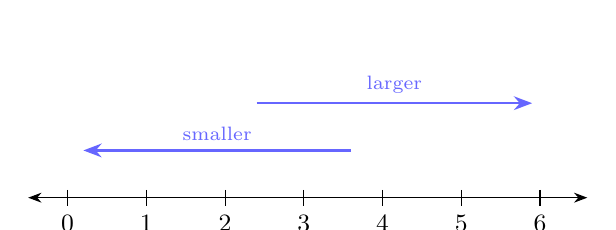
\begin{tikzpicture}[>=Stealth]
  \draw[<->] (-0.5,0) -- (6.6,0);
  \foreach \x in {0,...,6}{\draw (\x,0.1) -- (\x,-0.1) node[below] {\small$\x$};}
  \draw[->,blue!60,thick] (3.6,0.6) -- (0.2,0.6) node[midway,above] {\scriptsize smaller};
  \draw[->,blue!60,thick] (2.4,1.2) -- (5.9,1.2) node[midway,above] {\scriptsize larger};
\end{tikzpicture}
\end{center}

\begin{keybox}
The point labeled $0$ is called the \textbf{origin}. The points are equally spaced to the right of $0$ and labeled with the counting numbers. When a number is paired with a point, it is called the \textbf{coordinate} of the point.
\end{keybox}

\exbox{1} Which of the following are (a) counting numbers? (b) whole numbers? \seesol{1}
\[0,\ \tfrac14,\ 3,\ 5.2,\ 15,\ 105\]

\exbox{2} Which of the following are (a) counting numbers? (b) whole numbers? \seesol{2}
\[2.7,\ 5,\ -3,\ 0,\ \tfrac25,\ 16\]

\exbox{3} Which of the following are (a) counting numbers? (b) whole numbers? \seesol{3}
\[-2.5,\ 8,\ 207,\ 0,\ 4.7,\ \tfrac92,\ 97\]

\pagebreak
\subsection{Examples}

\solsec{1}
$a.$ The counting numbers start at $1$, so $0$ is not a counting number. The counting numbers are $3$, $15$ and $105$.\\
$b.$ Whole numbers are the counting numbers and $0$. The whole numbers are $0$, $3$, $15$ and $105$.\\
$\frac14$ and $5.2$ are neither counting numbers nor whole numbers. We will discuss these numbers later.

\solsec{2}
$a.$ Counting numbers: $5$ and $16$.\\
$b.$ Whole numbers: $0$, $5$ and $16$.\\
$2.7$, $-3$ and $\frac25$ are neither.

\solsec{3}
$a.$ Counting numbers: $8$, $207$ and $97$.\\
$b.$ Whole numbers: $0$, $8$, $207$ and $97$.\\
$-2.5$, $4.7$ and $\frac92$ are neither.
\clearpage
\def\chp{arith}
\lfoot{}
\section{Arithmetic Review}
%=====================================================================
\subsection{Number Sets}

In mathematics, a collection of numbers is called a \textbf{set}. For the beginning of this class we will only be concerned with two kinds of number sets.

\textbf{Counting numbers} (or \textbf{natural numbers}): positive numbers without fractions or decimals.
\[\{1,2,3,\ldots\}\]
\textbf{Whole numbers} (counting numbers and $0$):
\[\{0,1,2,3,\ldots\}\]

\begin{keybox}
Curly brackets $\{\ \}$ are used in math to group together numbers in a set. An ellipsis $\ldots$ means ``and so on'', meaning the numbers continue.
\end{keybox}

We can also denote a set with a \textbf{number line}: a straight line with equally spaced markings. Like the ellipsis, the arrow indicates the numbers continue.

\begin{center}
\begin{tikzpicture}[>=Stealth]
  \draw[->] (-0.2,0) -- (8.2,0);
  \foreach \x in {0,...,7}{\draw (\x,0.1) -- (\x,-0.1) node[below] {\small$\x$};}
\end{tikzpicture}
\end{center}

%=====================================================================
\subsection{Exponents}

Sometimes we need to multiply a number, and sometimes we need to multiply the same number multiple times. Clever mathematicians have created a simple way to denote this, called \textbf{exponents}.

If we want to multiply the number $2$ four times, instead of writing $2\times2\times2\times2$ we can simplify it to $2^4$. The way we would read this out loud is ``two to the fourth power''. In this case $4$ is called the \textbf{exponent} and $2$ is called the \textbf{base}.

\begin{keybox}
\textbf{Base} --- the number being multiplied.\\
\textbf{Exponent} --- the number of times the base is being multiplied.
\[\text{Written like: }\ \underset{\text{base}}{a}\!{}^{\,\overset{\text{exponent}}{b}}\]
\end{keybox}

\exbox{1} For the following examples, what is the base and what is the exponent? How would we say it? \seesol{1}
\begin{center}
$a.\ 3^2\qquad b.\ 3^3\qquad c.\ 2^5$
\end{center}

For the second and third powers there is another way we can say it. For something to the second power we can say it is ``squared''. For something to the third power we can say it is ``cubed''. These terms come from dimensionality: a square has \textbf{two} dimensions and a cube has \textbf{three} dimensions.

\begin{center}
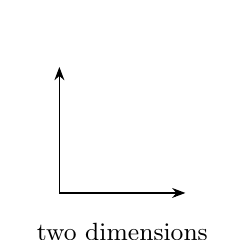
\begin{tikzpicture}[>=Stealth]
  \draw[->] (0,0) -- (1.6,0); \draw[->] (0,0) -- (0,1.6);
  \node at (0.8,-0.5) {\small two dimensions};
\end{tikzpicture}
\qquad\qquad
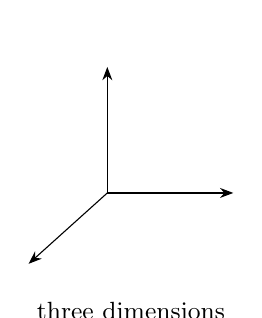
\begin{tikzpicture}[>=Stealth]
  \draw[->] (0,0) -- (1.6,0); \draw[->] (0,0) -- (0,1.6); \draw[->] (0,0) -- (-1,-0.9);
  \node at (0.3,-1.5) {\small three dimensions};
\end{tikzpicture}
\end{center}

Now that we know what exponents are, let's solve some.

\exbox{2} Expand and solve. \seesol{2}
\begin{center}
$a.\ 3^2\qquad b.\ 4^2\qquad c.\ 3^3\qquad d.\ 2^4$
\end{center}
For example, $3^3=3\cdot3\cdot3=9\cdot3=27$ and $2^4=2\cdot2\cdot2\cdot2=4\cdot4=16$. (Another way to check $3\cdot3=9$ is to add: $3+3+3=6+3=9$.)

\subsubsection*{Special Cases}

Let's look at some special cases of exponents, specifically when the exponent is $0$ or $1$.

\begin{keybox}
When the exponent is $1$ the answer is equal to the base.
\[a^1=a\qquad\text{for example }2^1=2,\quad7^1=7,\quad2437^1=2437\]
When the exponent is $0$ the answer is always $1$.
\[a^0=1\qquad\text{for example }7^0=1,\quad2437^0=1\]
\end{keybox}

\exbox{3} Let's do some examples. \seesol{3}
\begin{center}
$a.\ 5^1\qquad b.\ 9^1\qquad c.\ 4^0\qquad d.\ 8^0$
\end{center}

%=====================================================================
\subsection{Order of Operations}

Before we can specify an order, let's discuss what we mean by \textbf{operation}.

\begin{keybox}
An \textbf{operation} is something we do to a number or numbers. For example addition $+$, subtraction $-$, multiplication $\cdot$, division $\div$, as well as grouping $(\ )$ and $[\ ]$.
\end{keybox}

Does order really matter? Consider the expression $4+5\cdot2$. What answer do we get if we start with $4+5$ and then multiply by $2$? $4+5=9$ and $9\cdot2=18$. Now what happens if we do $5\cdot2$ first and then add $4$? $5\cdot2=10$ and $10+4=14$. We have two different answers for the same expression depending on the order we solve the parts, so we can confidently say \textbf{order matters}.

In math there is a specific order that we solve the operations in an expression. We remember it as \textbf{PEMDAS}:

\begin{keybox}
\textbf{P}arentheses $(\ )$ $[\ ]$ (inner to outer)\\
\textbf{E}xponents $a^b$\\
\textbf{M}ultiplication / \textbf{D}ivision (moving from left to right)\\
\textbf{A}ddition / \textbf{S}ubtraction (moving from left to right)
\end{keybox}

Let's look at our expression again, $4+5\cdot2$, and go down the list.

P? No parentheses. \quad E? No exponents. \quad M/D? Yes, $5\cdot2=10$, so the expression becomes $4+10$. \quad A/S? Yes, $4+10=14$. So we know $14$ is the correct answer.

\textbf{Example.} $4\cdot8-2\cdot6$.\\
P? No. E? No. M/D? Yes, $4\cdot8$ and $2\cdot6$. We go from left to right, so we do $4\cdot8=32$ and then $2\cdot6=12$. Now we have $32-12$. A/S? $32-12=20$.

\textbf{Example.} $5+2\cdot(7-1)$.\\
P? Yes, $(7-1)=6\to5+2\cdot6$. E? No. M/D? Yes, $2\cdot6=12\to5+12$. A/S? $5+12=17$.

\textbf{Example.} $3+2[10-3(5-2)]$.\\
P? Yes, $[10-3(5-2)]$ and $(5-2)$. Move from inner to outer, so $(5-2)=3\to[10-3(3)]\to[10-9]\to[1]\to3+2[1]$. E? No. M/D? $2[1]=2\to3+2$. A/S? $3+2=5$.

\subsubsection*{More Practice}

\textbf{Example.} $2+7\cdot6+8(4-6)$
\begin{align*}
  &=2+7\cdot6+8(-2)\\
  &=2+42+8(-2)=2+42+(-16)\\
  &=44-16=28
\end{align*}

\textbf{Example.} $-2^3+5(3-9+2^4)$
\begin{align*}
  &=-2^3+5(3-9+16)=-2^3+5(-6+16)\\
  &=-2^3+5(10)\\
  &=-8+5(10)=-8+50=42
\end{align*}

\textbf{Example.} $7-24\div8\times4+6$
\[7-3\times4+6=7-12+6=-5+6=1\]

\textbf{Example.} $-1\times[(3-4\times7)\div5]-2\times24\div6$
\begin{align*}
  &=-1\times[(3-28)\div5]-2\times24\div6\\
  &=-1\times[(-25)\div5]-2\times24\div6\\
  &=-1\times[-5]-2\times24\div6\\
  &=5-2\times24\div6=5-48\div6=5-8=-3
\end{align*}

\textbf{Example.} $-4(10^2)+20\div(-4)$
\[-4(100)+20\div(-4)=-400+(-5)=-400-5=-405\]

\textbf{Example.} $(3\times5^2\div15)-(5-2^2)$
\[(3\times25\div15)-(5-4)=(75\div15)-(1)=(5)-(1)=4\]

\textbf{Example.} $5(-12+7)\cdot3^2$
\[5(-5)\cdot9=-25\cdot9=-225\]

\textbf{Example.} $6(-3)(-2)=-18(-2)=36$.

\textbf{Example.} $\dfrac{-15+5(-4)}{12-17}$. Simplify the top and bottom separately:
\[\frac{-15+(-20)}{12-17}=\frac{-15-20}{12-17}=\frac{-35}{-5}=7\]

%=====================================================================
\subsection{Negative Numbers and Order Relations}

Say you have $\$20$ in a bank account and you draw $\$30$ from it. How much money will you have in your bank account? $-\$10$. When you subtract a larger number from a smaller number the result is negative.

\begin{keybox}
\textbf{Negative numbers} are numbers below zero. They can be represented on a number line. The set of numbers $\{\ldots,-3,-2,-1,0,1,2,3,\ldots\}$ is called the \textbf{integers}. Negative and positive numbers are \textbf{inverses} of each other.
\end{keybox}

\begin{center}
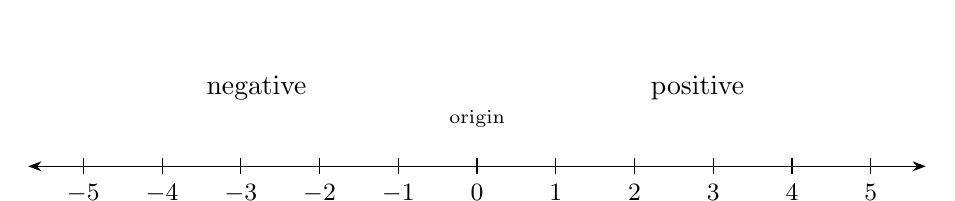
\begin{tikzpicture}[>=Stealth]
  \draw[<->] (-5.7,0) -- (5.7,0);
  \foreach \x in {-5,...,5}{\draw (\x,0.1) -- (\x,-0.1) node[below] {\small$\x$};}
  \node at (-2.8,1) {negative};
  \node at (2.8,1) {positive};
  \node[font=\scriptsize] at (0,0.6) {origin};
\end{tikzpicture}
\end{center}

A number to the \textbf{left} of another number is said to be \textbf{less than}. $1$ is less than $2$ $(1<2)$. $-5$ is less than $-3$ $(-5<-3)$. A number to the \textbf{right} of another is \textbf{greater than}. $3$ is greater than $2$ $(3>2)$. $-1$ is greater than $-2$ $(-1>-2)$.

So if $a$ is greater than $b$ we write $a>b$, and if $a$ is less than $b$ we write $a<b$. The further a negative number is from zero, the lesser it is.

\exbox{4} Fill in the blank with $<$ or $>$. \seesol{4}
\begin{center}
$a.\ 27\ \_\ 109\qquad b.\ 12\ \_\ 7\qquad c.\ -7\ \_\ 9\qquad d.\ -5\ \_\ -14$
\end{center}

\textbf{Review.} $7<12$ (7 is less than 12), $21>5$ (21 is greater than 5), and $-5<-3$ ($-5$ is less than $-3$).

\subsubsection*{Some Properties of Negative Numbers}

Multiplying a negative and a positive number gives us a negative number: $-a\times b=-(ab)$. Multiplying two negative numbers gives us a positive number: $-a\times-b=ab$. (More on these in the section on multiplication.)

%=====================================================================
\subsection{Absolute Value}

\begin{keybox}
The \textbf{absolute value} of a number is its distance from zero on the number line. It is never negative. We write $|a|$.\\
\textbf{Inverse numbers} have the same absolute value.
\end{keybox}

\begin{center}
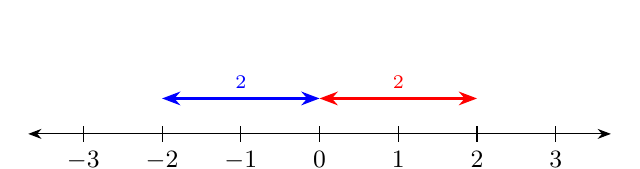
\begin{tikzpicture}[>=Stealth]
  \draw[<->] (-3.7,0) -- (3.7,0);
  \foreach \x in {-3,...,3}{\draw (\x,0.1) -- (\x,-0.1) node[below] {\small$\x$};}
  \draw[<->,thick,red] (0,0.45) -- (2,0.45) node[midway,above] {\scriptsize$2$};
  \draw[<->,thick,blue] (-2,0.45) -- (0,0.45) node[midway,above] {\scriptsize$2$};
\end{tikzpicture}
\end{center}
\[|2|=2\qquad\qquad|-2|=2\]

\exbox{5} Find the absolute value. \seesol{5}
\begin{center}
$a.\ |37|\qquad b.\ |-56|\qquad c.\ |-69|\qquad d.\ |-48|\qquad e.\ |9|\qquad f.\ |12|$
\end{center}

%=====================================================================
\subsection{Addition}

For any two numbers $a$ and $b$, the \textbf{sum} is $a+b$.

\subsubsection*{Properties of Addition}

\begin{keybox}
\textbf{Commutative property.} If $a$ and $b$ are any two numbers then
\[a+b=b+a\]
In other words, changing the order of two numbers in a sum doesn't change the result.\\[6pt]
\textbf{Associative property.} If $a$, $b$ and $c$ are any three numbers then
\[(a+b)+c=a+(b+c)\]
In other words, changing the grouping of three numbers doesn't change the result.\\[6pt]
\textbf{Addition property of $0$.} If $a$ is any number then
\[a+0=a\qquad\text{and}\qquad0+a=a\]
Adding $0$ to any number leaves that number unchanged.
\end{keybox}

\exbox{6} Rewrite each sum. \seesol{6}\\
\textbf{1.} Using the commutative property:
\begin{center}
$a.\ 2+7\qquad b.\ 12+7\qquad c.\ 15+0\qquad d.\ 6+n$
\end{center}
\textbf{2.} Using the associative property:
\begin{center}
$a.\ (12+15)+8\qquad b.\ (32+5)+1\qquad c.\ (13+4)+6\qquad d.\ (9+3)+7$
\end{center}

\exbox{7} Find each sum, using the properties to group numbers that are easy to add. \seesol{7}
\begin{center}
$a.\ 3+5+7\qquad b.\ 2+8+6\qquad c.\ 5+6+7+8+9\qquad d.\ 9+3+2+7+1$
\end{center}

\subsubsection*{Adding Positive and Negative Numbers}

\begin{keybox}
For the \textbf{same sign}, add the numbers and keep the sign:
\[a+b\qquad\qquad(-a)+(-b)=-(a+b)\]
For \textbf{opposite signs}, subtract the smaller from the larger and keep the sign of the larger:
\[-a+b=-(a-b)\ \text{ or }\ b-a\qquad\qquad a+(-b)=a-b\]
\end{keybox}

Adding a negative number is the same as subtracting the opposite.
\[a+(-b)=a-b\]
Subtracting a negative number is the same as adding the opposite.
\[a-(-b)=a+b\]
\[a-b=-(b-a)\]

\textbf{Example.} $10+(-5)+(-3)+4$
\[10-5+(-3)+4=5+(-3)+4=5-3+4=2+4=6\]

\textbf{Example.} $[-3+(-10)]+[8+(-2)]$
\[[-3-10]+[8-2]=[-13]+[6]=-7\]

\textbf{Review.} $10+(-15)+7$: $10-15+7=-5+7=7-5=2$.

Find the sum of $-12$, $-4$, and $8$: $-12+(-4)+8=-12-4+8=-16+8=-8$.

Find the sum of $9$, $11$, and $-24$: $9+11+(-24)=9+11-24=20-24=-4$.

\textbf{Application.} It was $12^\circ$F and the temperature drops by $14^\circ$F. What temperature is it now? $12^\circ\text{F}-14^\circ\text{F}=-2^\circ\text{F}$.

\subsubsection*{Subtraction}

\begin{keybox}
The \textbf{difference} of two numbers $a$ and $b$ is $a-b$. Subtraction is the same as adding the opposite:
\[a-b=a+(-b)\]
For any three numbers $a$, $b$, $c$: if $a-b=c$ then $b+c=a$.
\end{keybox}

For example, if $8-3=5$ then $3+5=8$.

%=====================================================================
\subsection{Multiplication}

If we have any two numbers $a$ and $b$ and we multiply them, the result is called the \textbf{product}.
\[a\cdot b=c\qquad c\text{ is the product}\]

\subsubsection*{Properties of Multiplication}

\begin{keybox}
\textbf{Commutative property.} $a\cdot b=b\cdot a$. Changing the order does not change the product.
\[5\cdot3=3\cdot5\quad\to\quad15=15\]
\textbf{Associative property.} $a\cdot(b\cdot c)=(a\cdot b)\cdot c$. Changing the grouping does not change the product.
\[(2\cdot3)\cdot6=2\cdot(3\cdot6)\quad\to\quad6\cdot6=2\cdot18\quad\to\quad36=36\]
\textbf{Distributive property.} $a\cdot(b+c)=a\cdot b+a\cdot c$. Multiplication can be distributed over addition and subtraction.
\[2(3+4)=2\cdot3+2\cdot4\quad\to\quad2(7)=6+8\quad\to\quad14=14\]
\textbf{Identity property.} $a\times1=a$, for example $9\times1=9$. Any number multiplied by $1$ does not change the number.\\[4pt]
\textbf{Zero property.} $a\times0=0$, for example $5\times0=0$. Any number multiplied by zero is zero.
\end{keybox}

\textbf{Examples.}
\begin{itemize}[itemsep=2pt]
  \item Associative property: $(2\times7)\times9=14\times9=126$, and $2\times(7\times9)=2\times63=126$. Also $2\times(21\times3)=2\times63=126$ and $(2\times21)\times3=42\times3=126$.
  \item Commutative property: $4\times3=12=3\times4$; $\ 9\times2=18=2\times9$; $\ -3\times12=-36=12\times(-3)$; $\ 5\times7=35=7\times5$.
  \item Distributive property: $3(7+4)=21+12=33$ and $3(11)=33$; $\ 9(3+2)=27+18=45$ and $9(5)=45$.
  \item Identity property: $9\times1=9$; $\ 7\times1=7$; $\ -5\times1=-5$.
  \item Zero property: $11\times0=0$; $\ 32\times0=0$; $\ -72\times0=0$.
\end{itemize}

\subsubsection*{Multiplication with Negative Numbers}

\begin{keybox}
\[a\cdot(-b)=-(ab)\qquad-a\cdot b=-(ab)\qquad(-a)\cdot(-b)=ab\]
If both numbers have the \textbf{same sign} the result is \textbf{positive}. If they have \textbf{opposite signs} the result is \textbf{negative}.
\end{keybox}

Why? Multiplication is repeated addition. $3\cdot5=5+5+5=15$ and
\[3\cdot(-5)=(-5)+(-5)+(-5)=-5-5-5=-15\]
and $-3\cdot(-5)=-(-5)-(-5)-(-5)=+5+5+5=15$.

\textbf{Example.} $a.\ 2(4)\quad b.\ -2(-4)\quad c.\ 2(-4)\quad d.\ -2(4)$
\begin{align*}
  a.\ 2(4)&=4+4=8\\
  b.\ -2(-4)&=-(-2)-(-2)-(-2)-(-2)=2+2+2+2=8\\
  c.\ 2(-4)&=-(2)-(2)-(2)-(2)=-4-4=-8\\
  d.\ -2(4)&=(-2)+(-2)+(-2)+(-2)=-2-2-2-2=-8
\end{align*}

\textbf{Example.} Simplify.
\begin{align*}
  a.\ -4(3)(-5)&=-12(-5)=60\\
  b.\ -3(2)(-1)&=-6(-1)=6\\
  c.\ -4+5(-6+2)&=-4+5(-4)=-4+(-20)=-4-20=-24\\
  d.\ -3(2-9)+4(-7-2)&=-3(-7)+4(-9)=21+(-36)=21-36=-15
\end{align*}

%=====================================================================
\subsection{Division}

\subsubsection*{Properties of Division}

\begin{keybox}
In $\dfrac ab=c$, $a$ is the \textbf{dividend}, $b$ is the \textbf{divisor} and $c$ is the \textbf{quotient}.\\[6pt]
Dividing by $1$ leaves a number unchanged: $a\div1=a$.\\[6pt]
Multiplying the top and bottom by the same number gives an equivalent fraction (for $n\neq0$):
\[\frac ab=\frac{na}{nb}\qquad\text{for example}\qquad\frac21=\frac42=\frac84\]
\end{keybox}

\subsubsection*{Division with Negative Numbers}

For $a$ and $b$, if $a\div b=c$ then $b\cdot c=a$. This is how we know the sign rules:
\begin{align*}
  6\div3&=2&\text{because }3\cdot2&=6\\
  6\div(-3)&=-2&\text{because }-3\cdot(-2)&=6\\
  -6\div3&=-2&\text{because }3\cdot(-2)&=-6\\
  -6\div(-3)&=2&\text{because }-3\cdot2&=-6
\end{align*}

\begin{keybox}
For numbers $a$ and $b$ where $b$ is \textbf{not} equal to zero:
\[-a\div b=-(a\div b)\qquad a\div(-b)=-(a\div b)\qquad-a\div(-b)=a\div b\]
\[\frac{-a}b=\frac a{-b}=-\left(\frac ab\right)\qquad\qquad\frac{-a}{-b}=\frac ab\]
\end{keybox}

\exbox{8} Divide. \seesol{8}
\begin{center}
$a.\ 12\div4\quad b.\ -12\div4\quad c.\ 12\div(-4)\quad d.\ -12\div(-4)$
\end{center}
\begin{center}
$a.\ \dfrac{20}5\qquad b.\ \dfrac{-20}5\qquad c.\ \dfrac{20}{-5}\qquad d.\ \dfrac{-20}{-5}$
\end{center}

\subsubsection*{Long Division Practice}

\exbox{9} Divide using long division, then check your answer by multiplying. \seesol{9}
\begin{center}
$a.\ 6750\div5\quad b.\ 50{,}400\div3\quad c.\ 1440\div32$\\[4pt]
$d.\ 227{,}920\div56\quad e.\ 9380\div35\quad f.\ 23{,}072\div32$
\end{center}

\exbox{10} More long division. \seesol{10}
\begin{center}
$a.\ 465\div5\quad b.\ 595\div7\quad c.\ 384\div12\quad d.\ 294\div14$
\end{center}

%=====================================================================
\subsection{Simplifying Algebraic Expressions}

\subsubsection*{The Associative Property}

\[4(5x)=(4\cdot5)x=20x\]
\begin{keybox}
Associative property: $(a+b)+c=a+(b+c)$ and $(a\cdot b)\cdot c=a\cdot(b\cdot c)$.
\end{keybox}

\textbf{Examples.}
\begin{align*}
  a.\ -2(5x)&=(-2\cdot5)x=-10x\\
  b.\ 3(-4y)&=(3\cdot(-4))y=-12y\\
  c.\ (2x+5)+10&=2x+(5+10)=2x+15
\end{align*}

\subsubsection*{The Distributive Property}

\[a(b+c)=ab+ac\]
\textbf{Examples.}
\begin{align*}
  a.\ 2(a-3)&=2a-(2\cdot3)=2a-6\\
  b.\ 4(5x+3)&=(4\cdot5x)+(4\cdot3)=20x+12\\
  c.\ 5(2x+3y)&=(5\cdot2x)+(5\cdot3y)=10x+15y
\end{align*}

\subsubsection*{Similar Terms}

\begin{keybox}
\textbf{Similar terms} have the same variable, for example $4x$ and $3x$. We combine them by adding the numbers in front.
\end{keybox}
\begin{align*}
  a.\ 4x+3x&=(4+3)x=7x\\
  b.\ 7a+a&=(7+1)a=8a\\
  c.\ -5x+7x&=(-5+7)x=2x\\
  d.\ 8y-y&=(8-1)y=7y\\
  e.\ -4a-2a&=(-4-2)a=-6a\\
  f.\ 3x-7x&=(3-7)x=-4x
\end{align*}

\subsubsection*{Area and Perimeter}

\begin{center}
\begin{tikzpicture}
  \draw (0,0) rectangle (2,2);
  \node[left] at (0,1) {$s$}; \node[below] at (1,0) {$s$};
  \node at (1,-1) {Area $=s^2$};\node at (1,-1.5) {Perimeter $=4s$};
  \draw (5,0.3) rectangle (9,2);
  \node[left] at (5,1.15) {$w$}; \node[below] at (7,0.3) {$l$};
  \node at (7,-1) {$A=l\cdot w$};\node at (7,-1.5) {$P=2l+2w$};
\end{tikzpicture}
\end{center}

%=====================================================================
\subsection{Summary}

\textbf{I. Number sets.} Counting numbers $\{1,2,3,\ldots\}$ and whole numbers $\{0,1,2,3,\ldots\}$.

\textbf{II. Order of operations.} To simplify a mathematical expression:
\begin{enumerate}[itemsep=0pt]
  \item Begin with expressions inside parentheses $(\ )$ $[\ ]$.
  \item Evaluate exponents.
  \item Multiplication and division from left to right.
  \item Addition and subtraction from left to right.
\end{enumerate}

\textbf{III. Exponents.} The base is the number being multiplied and the exponent is the number of times it is being multiplied. $a^0=1$ and $a^1=a$.

\textbf{IV. Absolute value.} The distance from $0$ on the number line. It is never negative.

\textbf{V. Addition and multiplication.}
\begin{itemize}[itemsep=0pt]
  \item Commutative property: of addition $a+b=b+a$, of multiplication $a\cdot b=b\cdot a$.
  \item Associative property: of addition $(a+b)+c=a+(b+c)$, of multiplication $(a\cdot b)\cdot c=a\cdot(b\cdot c)$.
  \item Distributive property: $a(b+c)=ab+ac$.
\end{itemize}

\textbf{VI. Addition of positive and negative numbers.} For the same sign, add them: $a+b$ and $(-a)+(-b)=-(a+b)$. For opposite signs, subtract: $-a+b=-(a-b)$ and $a+(-b)=a-b$.

\textbf{VII. Subtraction.} $a-b=a+(-b)$.

%=====================================================================

\subsection{Extra Practice}

The following extra problems come from the typed notes on exponents and negative numbers.

\exbox{11} For the following problems, identify the base, the exponent, and how it is said. \seesol{11}
\begin{center}
$a.\ 3^5\qquad b.\ 5^7\qquad c.\ 4^2\qquad d.\ 9^3$
\end{center}

\exbox{12} For the following problems, solve the expressions. \seesol{12}
\begin{center}
$a.\ 21^1\qquad b.\ 12^1\qquad c.\ 23^0\qquad d.\ 7^0$
\end{center}

\exbox{13} For the following problems choose the correct symbol $>$ or $<$. \seesol{13}
\begin{center}
$a.\ 3\ \_\ 5\qquad b.\ -5\ \_\ -7\qquad c.\ 4\ \_\ 2\qquad d.\ -9\ \_\ 3$
\end{center}

\pagebreak
\subsection{Examples}

\solsec{1}
$a.$ $3^2$: base $3$, exponent $2$, ``three to the second power'' or ``three squared''.\\
$b.$ $3^3$: base $3$, exponent $3$, ``three to the third power'' or ``three cubed''.\\
$c.$ $2^5$: base $2$, exponent $5$, ``two to the fifth power''.

\solsec{2}
$a.\ 3\cdot3=9\qquad b.\ 4\cdot4=16\qquad c.\ 3\cdot3\cdot3=9\cdot3=27\qquad d.\ 2\cdot2\cdot2\cdot2=4\cdot4=16$

\solsec{3}
$a.\ 5^1=5\qquad b.\ 9^1=9\qquad c.\ 4^0=1\qquad d.\ 8^0=1$

\solsec{4}
$a.\ 27<109\qquad b.\ 12>7\qquad c.\ -7<9\qquad d.\ -5>-14$

\solsec{5}
$a.\ 37\qquad b.\ 56\qquad c.\ 69\qquad d.\ 48\qquad e.\ 9\qquad f.\ 12$

\solsec{6}
\textbf{1.} Commutative: $a.\ 2+7=7+2\qquad b.\ 12+7=7+12\qquad c.\ 15+0=0+15\qquad d.\ 6+n=n+6$\\
\textbf{2.} Associative:
\begin{align*}
  a.\ (12+15)+8&=12+(15+8)&b.\ (32+5)+1&=32+(5+1)\\
  c.\ (13+4)+6&=13+(4+6)&d.\ (9+3)+7&=9+(3+7)
\end{align*}

\solsec{7}
\begin{align*}
  a.\ 3+5+7&=8+7=15\\
  b.\ 2+8+6&=10+6=16\\
  c.\ 5+6+7+8+9&=11+7+8+9=18+8+9=26+9=35\\
  d.\ 9+3+2+7+1&=12+2+7+1=14+7+1=21+1=22
\end{align*}

\solsec{8}
$a.\ 3\qquad b.\ -3\qquad c.\ -3\qquad d.\ 3$\\
$a.\ 4\qquad b.\ -4\qquad c.\ -4\qquad d.\ 4$

\solsec{9}
$a.\ 1350$ (check: $5\cdot1350=6750$)\\
$b.\ 16{,}800$ (check: $3\cdot16{,}800=50{,}400$)\\
$c.\ 45$ (check: $32\cdot45=1440$)\\
$d.\ 4070$ (check: $56\cdot4070=227{,}920$)\\
$e.\ 268$ (check: $35\cdot268=9380$)\\
$f.\ 721$ (check: $32\cdot721=23{,}072$)

\solsec{10}
$a.\ 93$ (check: $5\cdot93=465$)\\
$b.\ 85$ (check: $7\cdot85=595$)\\
$c.\ 32$ (check: $12\cdot32=384$)\\
$d.\ 21$ (check: $14\cdot21=294$)

\solsec{11}
$a.$ The base is $3$ and the exponent is $5$: ``three to the fifth power''.\\
$b.$ The base is $5$ and the exponent is $7$: ``five to the seventh power''.\\
$c.$ The base is $4$ and the exponent is $2$: ``four to the second power'' or ``four squared''.\\
$d.$ The base is $9$ and the exponent is $3$: ``nine to the third power'' or ``nine cubed''.

\solsec{12}
$a.\ 21^1=21\qquad b.\ 12^1=12\qquad c.\ 23^0=1\qquad d.\ 7^0=1$

\solsec{13}
$a.\ 3<5\qquad b.\ -5>-7\qquad c.\ 4>2\qquad d.\ -9<3$

\clearpage
\def\chp{div}
\source{Prealgebra}
\section{Divisibility Tests}
Another way to say that $375$ is a multiple of $5$ is to say that $375$ is \textbf{divisible} by $5$. In fact $375\div5=75$, so $375=5\cdot75$. On the other hand $10{,}519$ is not a multiple of $3$. When we divide $10{,}519$ by $3$ we do not get a counting number, so $10{,}519$ is not divisible by $3$.

\begin{keybox}
If a number $m$ is a multiple of $n$, then we say that $m$ is \textbf{divisible} by $n$.
\end{keybox}

Instead of dividing, we can use the following tests for some of the counting numbers between one and ten.

\begin{center}
\begin{tabular}{c|l}
A number is divisible by & \\\hline
$2$ & if the last digit is $0$, $2$, $4$, $6$ or $8$\\
$3$ & if the sum of the digits is divisible by $3$\\
$4$ & if the last two digits are divisible by $4$\\
$5$ & if the last digit is $0$ or $5$\\
$6$ & if the number is divisible by both $2$ and $3$\\
$8$ & if the last three digits are divisible by $8$\\
$9$ & if the sum of the digits is divisible by $9$\\
$10$ & if the last digit is $0$
\end{tabular}
\end{center}

\exbox{1} Determine whether $78$ is divisible by $2,3,4,5,6,8,9$ or $10$. \seesol{1}

\exbox{2} Determine whether $350$ is divisible by $2,3,4,5,6,8,9$ or $10$. \seesol{2}

\exbox{3} Determine whether $1{,}290$ is divisible by $2,3,4,5,6,8,9$ or $10$. \seesol{3}

\exbox{4} Determine whether $7{,}248$ is divisible by $2,3,4,5,6,8,9$ or $10$. \seesol{4}

\pagebreak
\subsection{Examples}

\renewcommand{\arraystretch}{1.25}

\solsec{1}
\begin{center}
\begin{tabular}{c|p{2.1in}|c|l}
By & Test & Divisible? & Check\\\hline
2 & Last digit $0,2,4,6,8$? Yes. & Yes & $78\div2=39$\\
3 & Sum of digits: $7+8=15$. Divisible by $3$? Yes. & Yes & $78\div3=26$\\
4 & Last two digits: $78\div4=19.5$. No. & No & $78\div4=19.5$\\
5 & Last digit $0$ or $5$? No. & No & $78\div5=15.6$\\
6 & Divisible by both $2$ and $3$? Yes. & Yes & $78\div6=13$\\
8 & Last three digits: $78\div8=9.75$. No. & No & $78\div8=9.75$\\
9 & Sum of digits $7+8=15$. Divisible by $9$? No. & No & $78\div9=8.\overline6$\\
10 & Last digit $0$? No. & No & $78\div10=7.8$
\end{tabular}
\end{center}
Thus $78$ is divisible by $2$, $3$ and $6$, but not $4$, $5$, $8$, $9$ or $10$.

\solsec{2}
\begin{center}
\begin{tabular}{c|p{2.1in}|c|l}
By & Test & Divisible? & Check\\\hline
2 & Last digit $0,2,4,6,8$? Yes. & Yes & $350\div2=175$\\
3 & Sum of digits: $3+5+0=8$. Divisible by $3$? No. & No & $350\div3=116.\overline6$\\
4 & Last two digits: $50\div4=12.5$. No. & No & $350\div4=87.5$\\
5 & Last digit $0$ or $5$? Yes. & Yes & $350\div5=70$\\
6 & Divisible by both $2$ and $3$? No. & No & $350\div6=58.\overline3$\\
8 & Last three digits: $350\div8=43.75$. No. & No & $350\div8=43.75$\\
9 & Sum of digits $3+5+0=8$. Divisible by $9$? No. & No & $350\div9=38.\overline8$\\
10 & Last digit $0$? Yes. & Yes & $350\div10=35$
\end{tabular}
\end{center}
Thus $350$ is divisible by $2$, $5$ and $10$, but not $3$, $4$, $6$, $8$ or $9$.

\solsec{3}
\begin{center}
\begin{tabular}{c|p{2.1in}|c|l}
By & Test & Divisible? & Check\\\hline
2 & Last digit $0,2,4,6,8$? Yes. & Yes & $1290\div2=645$\\
3 & Sum of digits: $1+2+9+0=12$. Divisible by $3$? Yes. & Yes & $1290\div3=430$\\
4 & Last two digits: $90\div4=22.5$. No. & No & $1290\div4=322.5$\\
5 & Last digit $0$ or $5$? Yes. & Yes & $1290\div5=258$\\
6 & Divisible by both $2$ and $3$? Yes. & Yes & $1290\div6=215$\\
8 & Last three digits: $290\div8=36.25$. No. & No & $1290\div8=161.25$\\
9 & Sum of digits $12$. Divisible by $9$? No. & No & $1290\div9=143.\overline3$\\
10 & Last digit $0$? Yes. & Yes & $1290\div10=129$
\end{tabular}
\end{center}
Thus $1{,}290$ is divisible by $2$, $3$, $5$, $6$ and $10$, but not $4$, $8$ or $9$.

\solsec{4}
\begin{center}
\begin{tabular}{c|p{2.1in}|c|l}
By & Test & Divisible? & Check\\\hline
2 & Last digit $0,2,4,6,8$? Yes. & Yes & $7248\div2=3624$\\
3 & Sum of digits: $7+2+4+8=21$. Divisible by $3$? Yes. & Yes & $7248\div3=2416$\\
4 & Last two digits: $48\div4=12$. Yes. & Yes & $7248\div4=1812$\\
5 & Last digit $0$ or $5$? No. & No & $7248\div5=1449.6$\\
6 & Divisible by both $2$ and $3$? Yes. & Yes & $7248\div6=1208$\\
8 & Last three digits: $248\div8=31$. Yes. & Yes & $7248\div8=906$\\
9 & Sum of digits $21$. Divisible by $9$? No. & No & $7248\div9=805.\overline3$\\
10 & Last digit $0$? No. & No & $7248\div10=724.8$
\end{tabular}
\end{center}
Thus $7{,}248$ is divisible by $2$, $3$, $4$, $6$ and $8$, but not $5$, $9$ or $10$.
\clearpage
\def\chp{frac}
\lfoot{}
\section{Fractions}
%=====================================================================
\subsection{The Meaning and Properties of Fractions}

A fraction is written
\[
  \frac{a}{b}\quad\begin{matrix}\leftarrow\text{ numerator}\\[-2pt]\leftarrow\text{ denominator}\end{matrix}
\]

\begin{keybox}
The \textbf{denominator} tells us how many equal parts the whole has been broken into.\\
The \textbf{numerator} tells us how many of those parts we are talking about.
\end{keybox}

A whole can be broken into many differently sized pieces. In Figure~\ref{fig:wall} one square is broken into pieces of size $\frac12$, $\frac14$, $\frac18$ and $\frac1{16}$.

\begin{figure}[h]
\centering
\begin{tikzpicture}[scale=1.1]
  \draw (0,0) rectangle (4,4);
  \draw (2,0) -- (2,4);
  \draw (0,2) -- (2,2);
  \draw (1,2) -- (1,4);
  \draw (0,3) -- (1,3);
  \node at (3,2) {$\frac12$};
  \node at (1,1) {$\frac14$};
  \node at (1.5,3) {$\frac18$};
  \node at (0.5,2.5) {\scriptsize$\frac1{16}$};
  \node at (0.5,3.5) {\scriptsize$\frac1{16}$};
\end{tikzpicture}
\caption{Pieces of a whole}\label{fig:wall}
\end{figure}

To visualize $\frac34$ we break a box into four equal pieces and shade three of them. To visualize $\frac59$ we break a circle into nine equal slices and shade five.

\begin{center}
$\dfrac34$\ \fracgrid{2}{2}{3}\qquad\qquad $\dfrac59$\ \fracpie{9}{5}
\end{center}

\exbox{1} Name the numerator and denominator. \seesol{1}

\begin{center}
$a.\ \dfrac34$\qquad $b.\ \dfrac5{12}$\qquad $c.\ \dfrac a{11}$\qquad $d.\ \dfrac91$
\end{center}

\subsubsection*{Proper and Improper Fractions}

\begin{keybox}
A fraction $\dfrac ab$ is a \textbf{proper fraction} if $a<b$. For example $\dfrac34,\ \dfrac18,\ \dfrac a{10}$ (when $a<10$).\\[4pt]
A fraction $\dfrac ab$ is an \textbf{improper fraction} if $a\geq b$. For example $\dfrac95,\ \dfrac{10}{10},\ \dfrac61$.
\end{keybox}

Fractions can be shown on a number line. Here the space from $0$ to $1$ is broken into four equal pieces of size $\frac14$. Each arrow starts at $0$ and shows $\frac14$, $\frac24$, $\frac34$ and $\frac44$.

\begin{center}
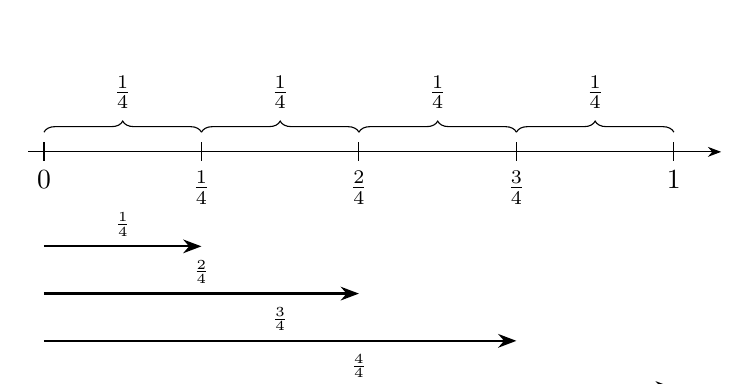
\begin{tikzpicture}[>=Stealth]
  \draw[->] (-0.2,0) -- (8.6,0);
  \foreach \x/\l in {0/0,2/\frac14,4/\frac24,6/\frac34,8/1}{
    \draw (\x,0.12) -- (\x,-0.12) node[below] {$\l$};
  }
  \foreach \x in {0,2,4,6}{
    \draw[decorate,decoration={brace,amplitude=4pt}] (\x,0.25) -- (\x+2,0.25) node[midway,above=5pt] {$\frac14$};
  }
  \draw[->,thick] (0,-1.2) -- (2,-1.2) node[midway,above] {\scriptsize$\frac14$};
  \draw[->,thick] (0,-1.8) -- (4,-1.8) node[midway,above] {\scriptsize$\frac24$};
  \draw[->,thick] (0,-2.4) -- (6,-2.4) node[midway,above] {\scriptsize$\frac34$};
  \draw[->,thick] (0,-3.0) -- (8,-3.0) node[midway,above] {\scriptsize$\frac44$};
\end{tikzpicture}
\end{center}

%=====================================================================

\subsection{Equivalent Fractions}

Look at the two squares below. Both have the same amount shaded, even though they are broken into different numbers of pieces.

\begin{center}
$\dfrac24$\ \fracgrid{2}{2}{2}\ $\;\;=\;\;$ $\dfrac12$\ \fracgrid{1}{2}{1}
\end{center}

The same is true for circles. $\frac26$ and $\frac13$ shade the same amount, and so does $\frac4{12}$:

\begin{center}
$\dfrac26$\ \fracpie{6}{2}\qquad $\dfrac13$\ \fracpie{3}{1}\qquad $\dfrac4{12}$\ \fracpie{12}{4}
\end{center}
\[
  \frac13=\frac26=\frac4{12}
\]
Fractions that name the same amount are called \textbf{equivalent fractions}.

\begin{keybox}
We can create an equivalent fraction by \textbf{multiplying} the numerator and denominator by the same non-zero number $n$:
\[\frac ab=\frac{a\cdot n}{b\cdot n}\]
We can also create an equivalent fraction by \textbf{dividing} the numerator and denominator by the same non-zero number $n$:
\[\frac ab=\frac{a\div n}{b\div n}\]
\end{keybox}

For example
\[
  \frac34=\frac{3\cdot5}{4\cdot5}=\frac{15}{20}
  \qquad\text{and}\qquad
  \frac34=\frac{3\cdot3x}{4\cdot3x}=\frac{9x}{12x}
  \qquad\text{and}\qquad
  \frac{10}{12}=\frac{10\div2}{12\div2}=\frac56.
\]

Two more facts we will use often: any number divided by $1$ is itself, and any (non-zero) number divided by itself is $1$.

\begin{keybox}
\[\frac a1=a\qquad\qquad \frac aa=1\quad(a\neq0)\]
\end{keybox}

\exbox{2} Write each fraction as a whole number. \seesol{2}

\begin{center}
$a.\ \dfrac91$\qquad $b.\ \dfrac99$\qquad $c.\ \dfrac{18}9$\qquad $d.\ \dfrac{27}9$
\end{center}

\exbox{3} Which of $\dfrac58,\ \dfrac56,\ \dfrac34,\ \dfrac23$ is the smallest? Write all four with a denominator of $24$ and then order them from smallest to largest. \seesol{3}

%=====================================================================

\subsection{Prime Numbers}

\begin{keybox}
A \textbf{prime number} is a whole number greater than $1$ that has exactly two divisors: itself and $1$. In other words, we cannot divide a prime by any other number and get a whole number back (without a remainder).\\[4pt]
Prime numbers: $\{2,3,5,7,11,\ldots\}$
\end{keybox}

\begin{keybox}
A \textbf{composite number} is a whole number greater than $1$ that is not a prime number. That is, there exists a number other than itself and $1$ that we can divide a composite number by and get a whole number.
\end{keybox}

\exbox{4} Identify each number as prime or composite. \seesol{4}

\begin{center}
$a.\ 17$\qquad\qquad $b.\ 12$
\end{center}

\subsubsection*{Prime Factorization}

Every composite number can be broken into prime numbers. One way to do this is with a \textbf{factor tree}: split the number into two factors and keep splitting any factor that is not prime. We circle the primes. Reading all of the circled primes gives the \textbf{prime factorization}.

For $12$:
\begin{center}
\ftree{12}{2/6,2/3}{2}
\qquad
$12=2\cdot2\cdot3=2^2\cdot3$
\end{center}

For $108$:
\begin{center}
\ftree{108}{2/54,2/27,3/9,3/3}{4}
\qquad
$\begin{aligned}108&=2\cdot2\cdot3\cdot3\cdot3\\&=2^2\cdot3^3\end{aligned}$
\end{center}

\exbox{5} Find the prime factorization of each number. Write your answer with exponents. \seesol{5}

\begin{center}
$a.\ 60$\qquad $b.\ 352$\qquad $c.\ 125$
\end{center}

Instead of a factor tree we can divide by primes over and over until we reach $1$ (or a prime). For instance $352\div2=176$, $176\div2=88$, and so on.

%=====================================================================

\subsection{Lowest Terms}

\begin{keybox}
A fraction is in \textbf{lowest terms} when its numerator and denominator have no factors in common (other than $1$).
\end{keybox}

If we divide the numerator and denominator by $2$,
\[
  \frac68=\frac{6\div2}{8\div2}=\frac34
\]
and $\frac34$ is the lowest term of $\frac68$.

Prime factorizations make it easy to find common factors. For $\frac{12}{15}$ we have $12=2\cdot2\cdot3$ and $15=3\cdot5$, so
\[
  \frac{12}{15}=\frac{2\cdot2\cdot\cancel{3}}{\cancel{3}\cdot5}=\frac45.
\]

\exbox{6} Reduce each fraction to lowest terms. \seesol{6}

\begin{center}
$a.\ \dfrac{20}{24}$\qquad $b.\ \dfrac6{42}$\qquad $c.\ \dfrac4{40}$\qquad $d.\ -\dfrac{105}{30}$\qquad $e.\ \dfrac{136}{24}$
\end{center}

%=====================================================================

\subsection{Multiplication with Fractions}

\begin{keybox}
\textbf{Rule.} The product of two fractions is a fraction whose numerator is the product of the two numerators and whose denominator is the product of the two denominators.
\[\frac ab\cdot\frac cd=\frac{a\cdot c}{b\cdot d}\]
\end{keybox}

\textbf{Example.}
\[\frac35\cdot\frac27=\frac{3\cdot2}{5\cdot7}=\frac6{35}\]

Remember $5=\dfrac51$, so a whole number can be multiplied with a fraction too.
\[\frac38\cdot5=\frac38\cdot\frac51=\frac{3\cdot5}{8\cdot1}=\frac{15}8\]

Parentheses first:
\[\frac12\left(\frac34\cdot\frac15\right)=\frac12\left(\frac3{20}\right)=\frac{1\cdot3}{2\cdot20}=\frac3{40}\]

When the numbers are larger, factor and cancel before multiplying.
\[
  \frac{15}8\cdot\frac49=\frac{3\cdot5}{2\cdot2\cdot2}\cdot\frac{2\cdot2}{3\cdot3}
  =\frac{\cancel3\cdot5\cdot\cancel2\cdot\cancel2}{\cancel2\cdot\cancel2\cdot2\cdot\cancel3\cdot3}=\frac5{2\cdot3}=\frac56
\]

With negative numbers the same sign rules apply (see \textbf{Negative Numbers}).
\[
  -\frac92\cdot\frac8{18}=-\frac{3\cdot3}{2}\cdot\frac{2\cdot2\cdot2}{2\cdot3\cdot3}=-\frac21=-2
\qquad
\left(-\frac34\right)^2=\left(-\frac34\right)\left(-\frac34\right)=\frac9{16}
\]

\subsubsection*{``Of'' means multiply}

\[
  \frac34\text{ of }12=\frac34\cdot\frac{12}1=\frac{3\cdot2\cdot2\cdot3}{2\cdot2\cdot1}=\frac91=9
\]
\[
  \frac25\text{ of }35=\frac25\cdot\frac{35}1=\frac{2\cdot7\cdot5}{5\cdot1}=\frac{14}1=14
\]

\subsubsection*{The Area of a Triangle}

Let $b$ be the base and $h$ the height of a triangle. Its area is
\[A=\frac12bh.\]

\begin{center}
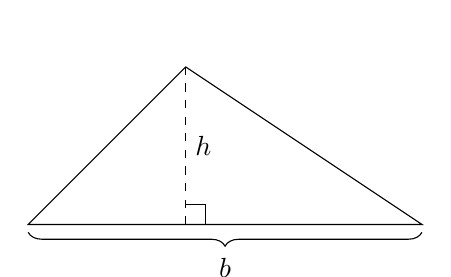
\begin{tikzpicture}
  \draw (0,0) -- (5,0) -- (2,2) -- cycle;
  \draw[dashed] (2,0) -- (2,2);
  \draw (2,0) ++(0,0.25) -- ++(0.25,0) -- ++(0,-0.25);
  \node[right] at (2,1) {$h$};
  \draw[decorate,decoration={brace,mirror,amplitude=5pt}] (0,-0.1) -- (5,-0.1) node[midway,below=6pt] {$b$};
\end{tikzpicture}
\end{center}

\textbf{Example.} A triangle has a base of $10$ in and a height of $7$ in.
\[A=\frac12(7\text{ in})(10\text{ in})=\frac12\cdot7\cdot2\cdot5=1\cdot7\cdot5=35\text{ in}^2\]

\textbf{Example.} A triangle has a base of $6$ in and a height of $5$ in.
\[A=\frac12\cdot5\cdot6=\frac12\cdot30=\frac{30}2=15\text{ in}^2\]

%=====================================================================

\subsection{Division with Fractions}

\subsubsection*{Reciprocals}

\begin{keybox}
Two numbers whose product is $1$ are said to be \textbf{reciprocals}. The reciprocal of $\dfrac ab$ is $\dfrac ba$ (for $a\neq0$, $b\neq0$).
\[\frac ab\cdot\frac ba=\frac{a\cdot b}{b\cdot a}=\frac{a\cdot b}{a\cdot b}=1\]
\end{keybox}

\[5\cdot\frac15=\frac51\cdot\frac15=\frac{5\cdot1}{1\cdot5}=1\qquad
\frac34\cdot\frac43=\frac{12}{12}=1\qquad
\frac78\cdot\frac87=\frac{56}{56}=1\]

\subsubsection*{Dividing Fractions}

\begin{keybox}
To divide by a fraction, multiply by its reciprocal.
\[\frac ab\div\frac cd=\frac ab\cdot\frac dc\]
\end{keybox}

\[
  \frac12\div\frac14=\frac12\cdot\frac41=\frac{1\cdot\cancel2\cdot2}{\cancel2\cdot1}=\frac21=2
\]
\[
  \frac38\div\frac94=\frac38\cdot\frac49=\frac{\cancel3\cdot\cancel2\cdot\cancel2}{\cancel2\cdot\cancel2\cdot2\cdot\cancel3\cdot3}=\frac1{2\cdot3}=\frac16
\]
\[
  \frac23\div2=\frac23\cdot\frac12=\frac{\cancel2\cdot1}{3\cdot\cancel2}=\frac13
\qquad
2\div\left(-\frac13\right)=\frac21\cdot\left(-\frac31\right)=\frac{2\cdot(-3)}{1\cdot1}=-6
\]
\[
  -\frac4{27}\div\frac{16}9=-\frac4{27}\cdot\frac9{16}=-\frac{2\cdot2\cdot3\cdot3}{3\cdot3\cdot3\cdot2\cdot2\cdot2\cdot2}=-\frac1{3\cdot2\cdot2}=-\frac1{12}
\]

\exbox{7} Divide. \seesol{7}

\begin{center}
$a.\ \dfrac{16}{35}\div8$\qquad\qquad $b.\ 27\div\dfrac32$\qquad\qquad $c.\ \dfrac9{32}\div\dfrac{27}8$
\end{center}

\subsubsection*{Order of Operations with Fractions}

The order of operations (see \textbf{Order of Operations}) works exactly the same with fractions.

\textbf{Example.} $\displaystyle\frac83\div\frac16+5$
\[
  \frac83\div\frac16+5=\frac83\cdot\frac61+5=\frac{2\cdot2\cdot2\cdot2\cdot\cancel3}{\cancel3\cdot1}+5=\frac{16}1+5=16+5=21
\]

\textbf{Example.} $\displaystyle\left[32\div\left(\frac43\right)^2\right]+\left[75\div\left(\frac52\right)^2\right]$

Exponents first, then divide inside each bracket, then add.
\begin{align*}
  &=\left[32\div\frac{16}9\right]+\left[75\div\frac{25}4\right]\\
  &=\left[32\cdot\frac9{16}\right]+\left[75\cdot\frac4{25}\right]\\
  &=\left[2\cdot9\right]+\left[3\cdot4\right]=18+12=30
\end{align*}

%=====================================================================

\subsection{Addition and Subtraction with Fractions}

Remember the distributive property:
\[a(b+c)=a(b)+a(c)\]
When we add fractions with the same denominator, we can factor out $\frac17$:
\[
  \frac27+\frac37=2\left(\frac17\right)+3\left(\frac17\right)=\frac17(2+3)=\frac17(5)=\frac51\cdot\frac17=\frac57
\]
Note that $a\cdot\dfrac1b=\dfrac a1\cdot\dfrac1b=\dfrac ab$.

\begin{keybox}
\textbf{Rule.} To add two fractions that have the same denominator, we add their numerators to get the numerator of the answer. The denominator is the same as the original fractions.
\[\frac ac+\frac bc=\frac{a+b}c\]
It is the same for subtraction.
\[\frac ac-\frac bc=\frac{a-b}c\]
\end{keybox}

\textbf{Examples.}
\[\frac38+\frac18=\frac{3+1}8=\frac48=\frac12\qquad
\frac95-\frac35=\frac{9-3}5=\frac65\qquad
\frac37+\frac27+\frac97=\frac{3+2+9}7=\frac{14}7=2\]

\subsubsection*{The Least Common Denominator}

\begin{keybox}
The \textbf{Least Common Denominator (LCD)} for a set of denominators is the smallest number that is exactly divisible by each denominator.
\end{keybox}

\textbf{Example.} Find the LCD for $\dfrac5{12}$ and $\dfrac7{18}$.

Factor each denominator: $12=2\cdot2\cdot3$ and $18=2\cdot3\cdot3$. The LCD uses each prime as many times as it appears in the denominator where it appears most:
\[\text{LCD}=2\cdot2\cdot3\cdot3=4\cdot9=36\]
Notice $36=12\cdot3$ and $36=18\cdot2$. So
\[
  \frac5{12}=\frac{5\cdot3}{12\cdot3}=\frac{15}{36}\qquad\frac7{18}=\frac{7\cdot2}{18\cdot2}=\frac{14}{36}
\]
\[
  \frac5{12}+\frac7{18}=\frac{15}{36}+\frac{14}{36}=\frac{15+14}{36}=\frac{29}{36}
\]

\begin{keybox}
\textbf{To add or subtract fractions with different denominators:}\\
\textbf{Step 1.} Factor the denominators.\\
\textbf{Step 2.} Rewrite each fraction as an equivalent fraction with the LCD as its denominator.\\
\textbf{Step 3.} Add or subtract the numerators of the equivalent fractions.\\
\textbf{Step 4.} Reduce the fraction.
\end{keybox}

\textbf{Example.} $\dfrac34+\dfrac16$. Here $4=2\cdot2$ and $6=2\cdot3$, so $\text{LCD}=2\cdot2\cdot3=12$.
\[\frac34+\frac16=\frac{3\cdot3}{4\cdot3}+\frac{1\cdot2}{6\cdot2}=\frac9{12}+\frac2{12}=\frac{11}{12}\]

\textbf{Example.} $\dfrac7{15}-\dfrac3{10}$. Here $15=3\cdot5$ and $10=2\cdot5$, so $\text{LCD}=3\cdot5\cdot2=30$.
\[\frac7{15}-\frac3{10}=\frac{14}{30}-\frac9{30}=\frac{14-9}{30}=\frac5{30}=\frac16\]

\textbf{Example.} $\dfrac35-\dfrac16$. The LCD is $5\cdot6=30$.
\[\frac35-\frac16=\frac{3\cdot6}{5\cdot6}-\frac{1\cdot5}{6\cdot5}=\frac{18}{30}-\frac5{30}=\frac{13}{30}\]

\textbf{Example.} $\dfrac16+\dfrac18+\dfrac14$. Here $6=2\cdot3$, $8=2\cdot2\cdot2$, $4=2\cdot2$, so $\text{LCD}=3\cdot2\cdot2\cdot2=24$.
\[\frac4{24}+\frac3{24}+\frac6{24}=\frac{4+3+6}{24}=\frac{13}{24}\]

\textbf{Example.} A whole number is a fraction over $1$: $3-\dfrac56=\dfrac31-\dfrac56=\dfrac{18}6-\dfrac56=\dfrac{13}6$.

\subsubsection*{With Negative Fractions}
\[\frac38+\left(-\frac18\right)=\frac{3+(-1)}8=\frac{3-1}8=\frac28=\frac14\]
\[
  \frac1{10}+\left(-\frac45\right)+\left(-\frac3{20}\right)
  =\frac2{20}+\left(-\frac{16}{20}\right)+\left(-\frac3{20}\right)
  =\frac{2-16-3}{20}=\frac{-17}{20}=-\frac{17}{20}
\]
\[-\frac35-\frac25=\frac{-3-2}5=\frac{-5}5=-1\]

\exbox{8} Find the LCD and write the fractions from smallest to largest. \seesol{8}

\begin{center}
$\dfrac58,\quad\dfrac5{16},\quad\dfrac34,\quad\dfrac12$
\end{center}

%=====================================================================

\subsection{Review Problems}

\begin{enumerate}[label=\arabic*.]
  \item Factor $48$ into its prime numbers.
  \item Reduce $\dfrac{45}{60}$ to lowest terms.
  \item Multiply $\dfrac{15}8\cdot\dfrac49$.
  \item Find the quotient of $(-2)$ and $\left(-\dfrac13\right)$.
  \item Simplify $\dfrac{48}{44}\div\left(-\dfrac4{11}\right)^2$ as much as possible.
  \item Simplify $\dfrac{\dfrac78-\dfrac12}{\dfrac14+\dfrac12}$.
  \item Subtract $\dfrac56$ from the product of $\dfrac32$ and $\dfrac23$.
  \item If the quotient of $18$ and $\dfrac35$ is increased by $10$, what number results?
  \item $\dfrac68-\dfrac28$
  \item $-\dfrac7{15}+\dfrac5{12}$
  \item Find the prime factorization of $22440$.
  \item Simplify $\left(\left[\left(\dfrac52\right)^3\div\dfrac52\right]-\left[\left(\dfrac32\right)^2\div\dfrac{45}8\right]\right)\div\dfrac{117}{10}$
\end{enumerate}
Also reduce: $\dfrac{210}{270}$ and $\dfrac{125}{370}$. \seesol{R}

%=====================================================================

\pagebreak
\subsection{Examples}

\solsec{1}
$a.$ Numerator $3$, denominator $4$.\quad $b.$ Numerator $5$, denominator $12$.\quad $c.$ Numerator $a$, denominator $11$.\quad $d.$ Numerator $9$, denominator $1$.

\solsec{2}
$a.\ \dfrac91=9\qquad b.\ \dfrac99=1\qquad c.\ \dfrac{18}9=2\qquad d.\ \dfrac{27}9=3$

\solsec{3}
Since $8\cdot3=24$, $6\cdot4=24$, $4\cdot6=24$, $3\cdot8=24$:
\[
  \frac{5\cdot3}{8\cdot3}=\frac{15}{24},\quad
  \frac{5\cdot4}{6\cdot4}=\frac{20}{24},\quad
  \frac{3\cdot6}{4\cdot6}=\frac{18}{24},\quad
  \frac{2\cdot8}{3\cdot8}=\frac{16}{24}
\]
\[\frac{15}{24}<\frac{16}{24}<\frac{18}{24}<\frac{20}{24}\qquad\Longrightarrow\qquad\frac58<\frac23<\frac34<\frac56\]
The smallest is $\dfrac58$.

\solsec{4}
$a.$ $17$ is not divisible by $2,3,5,7,11$ or $13$ (each leaves a remainder), so $17$ is \textbf{prime}.\\
$b.$ $\dfrac{12}2=6$ is a whole number, so $12$ is divisible by something other than itself and $1$. $12$ is \textbf{composite}.

\solsec{5}
$a.$ $60=2\cdot30=2\cdot3\cdot10=2\cdot3\cdot2\cdot5$, so $60=2^2\cdot3\cdot5$.\\
\hspace*{1.2em}\ftree{60}{2/30,3/10,2/5}{3}\\
$b.$ $352=2\cdot176=2\cdot2\cdot88=2\cdot2\cdot2\cdot44=2\cdot2\cdot2\cdot2\cdot22=2\cdot2\cdot2\cdot2\cdot2\cdot11$, so $352=2^5\cdot11$.\\
$c.$ $125=5\cdot25=5\cdot5\cdot5$, so $125=5^3$.

\solsec{6}
\begin{align*}
a.\ \frac{20}{24}&=\frac{2\cdot2\cdot5}{2\cdot2\cdot2\cdot3}=\frac5{2\cdot3}=\frac56\\
b.\ \frac6{42}&=\frac{2\cdot3}{2\cdot3\cdot7}=\frac17\\
c.\ \frac4{40}&=\frac{2\cdot2}{2\cdot2\cdot2\cdot5}=\frac1{2\cdot5}=\frac1{10}\\
d.\ -\frac{105}{30}&=-\frac{3\cdot5\cdot7}{2\cdot3\cdot5}=-\frac72\\
e.\ \frac{136}{24}&=\frac{2\cdot2\cdot2\cdot17}{2\cdot2\cdot2\cdot3}=\frac{17}3
\end{align*}

\solsec{7}
$a.\ \dfrac{16}{35}\cdot\dfrac18=\dfrac{2\cdot2\cdot2\cdot2\cdot1}{5\cdot7\cdot2\cdot2\cdot2}=\dfrac2{35}$\\[6pt]
$b.\ \dfrac{27}1\cdot\dfrac23=\dfrac{3\cdot3\cdot3\cdot2}{1\cdot3}=3\cdot3\cdot2=18$\\[6pt]
$c.\ \dfrac9{32}\cdot\dfrac8{27}=\dfrac{3\cdot3}{2\cdot2\cdot2\cdot2\cdot2}\cdot\dfrac{2\cdot2\cdot2}{3\cdot3\cdot3}=\dfrac1{2\cdot2}\cdot\dfrac13=\dfrac1{12}$

\solsec{8}
$8=2\cdot2\cdot2$, $16=2\cdot2\cdot2\cdot2$, $4=2\cdot2$, $2=2$, so $\text{LCD}=16$.
\[\frac58=\frac{10}{16},\quad\frac5{16},\quad\frac34=\frac{12}{16},\quad\frac12=\frac8{16}\]
\[\frac5{16}<\frac8{16}<\frac{10}{16}<\frac{12}{16}\qquad\Longrightarrow\qquad\frac5{16}<\frac12<\frac58<\frac34\]

\solsec{R}
\begin{enumerate}[label=\arabic*.]
  \item $48=2\cdot2\cdot2\cdot2\cdot3=2^4\cdot3$
  \item $\dfrac{45}{60}=\dfrac{3\cdot3\cdot5}{2\cdot2\cdot3\cdot5}=\dfrac34$
  \item $\dfrac{15}8\cdot\dfrac49=\dfrac56$ (see the multiplication section)
  \item $-2\div\left(-\dfrac13\right)=\dfrac{-2}1\cdot\dfrac{-3}1=\dfrac61=6$
  \item $\left(-\dfrac4{11}\right)^2=\dfrac{16}{121}$, so $\dfrac{48}{44}\cdot\dfrac{121}{16}=\dfrac{2\cdot2\cdot2\cdot2\cdot3}{2\cdot2\cdot11}\cdot\dfrac{11\cdot11}{2\cdot2\cdot2\cdot2}=\dfrac{3\cdot11}{2\cdot2}=\dfrac{33}4$
  \item Numerator: $\dfrac78-\dfrac48=\dfrac38$. Denominator: $\dfrac14+\dfrac24=\dfrac34$. Then $\dfrac38\div\dfrac34=\dfrac38\cdot\dfrac43=\dfrac12$.
  \item $\dfrac32\cdot\dfrac23-\dfrac56=1-\dfrac56=\dfrac66-\dfrac56=\dfrac16$
  \item $\left(18\div\dfrac35\right)+10=\dfrac{18}1\cdot\dfrac53+10=30+10=40$
  \item $\dfrac68-\dfrac28=\dfrac48=\dfrac{2\cdot2}{2\cdot2\cdot2}=\dfrac12$
  \item $\text{LCD}=5\cdot3\cdot2\cdot2=60$: $-\dfrac{28}{60}+\dfrac{25}{60}=\dfrac{-3}{60}=-\dfrac1{20}$
  \item $22440=10\cdot2244=2\cdot5\cdot2\cdot1122=2\cdot5\cdot2\cdot2\cdot561=2\cdot5\cdot2\cdot2\cdot3\cdot187=2\cdot5\cdot2\cdot2\cdot3\cdot11\cdot17$, so $22440=2^3\cdot3\cdot5\cdot11\cdot17$.
  \item $\left(\dfrac52\right)^3\div\dfrac52=\dfrac{125}8\cdot\dfrac25=\dfrac{25}4$ and $\left(\dfrac32\right)^2\div\dfrac{45}8=\dfrac94\cdot\dfrac8{45}=\dfrac25$.\\
  Then $\dfrac{25}4-\dfrac25=\dfrac{125}{20}-\dfrac8{20}=\dfrac{117}{20}$, and $\dfrac{117}{20}\div\dfrac{117}{10}=\dfrac{117}{20}\cdot\dfrac{10}{117}=\dfrac{10}{20}=\dfrac12$.
\end{enumerate}
Also: $\dfrac{210}{270}=\dfrac{3\cdot7\cdot2\cdot5}{3\cdot3\cdot3\cdot2\cdot5}=\dfrac79$ and $\dfrac{125}{370}=\dfrac{5\cdot5\cdot5}{2\cdot5\cdot37}=\dfrac{25}{74}$.
\clearpage
\def\chp{dec}
\lfoot{}
\section{Decimals and Percents}
%=====================================================================
\subsection{Mixed Notation}

Back when we began fractions, we used shaded boxes to visualize them. Consider the improper fraction $\frac74$. Each box is broken into four pieces, so we need two boxes to shade seven pieces:

\begin{center}
\fracgrid{2}{2}{4}\qquad\fracgrid{2}{2}{3}
\end{center}

We get one full box and one box that is $\frac34$ shaded. That is
\[\frac74=\frac44+\frac34=1+\frac34\]
and we write $\dfrac74=1\dfrac34$.

\begin{keybox}
We can turn improper fractions into a combination of a whole number and a proper fraction. This is called \textbf{mixed notation} (a \textbf{mixed number}).
\end{keybox}

Let's say we have the improper fraction $\frac{13}6$. We break the numerator into as many copies of the denominator as we can:
\[\frac{13}6\to\frac66+\frac76\to\frac66+\frac66+\frac16\to1+1+\frac16=2\frac16\]
So $\dfrac{13}6=2\dfrac16$.

\textbf{Example.} $\dfrac{11}4\to\dfrac44+\dfrac74\to\dfrac44+\dfrac44+\dfrac34\to1+1+\dfrac34=2\dfrac34$

\exbox{1} Write each improper fraction in mixed notation. \seesol{1}

\begin{center}
$a.\ \dfrac{10}3$\qquad $b.\ \dfrac95$\qquad $c.\ \dfrac{21}4$
\end{center}

%=====================================================================
\subsection{Introduction to Decimals}

Recall our sets of numbers:
\begin{align*}
  \textbf{Counting numbers}&\quad\{1,2,3,4,\ldots\}\\
  \textbf{Whole numbers}&\quad\{0,1,2,3,4,\ldots\}\\
  \textbf{Integers}&\quad\{\ldots,-4,-3,-2,-1,0,1,2,3,4,\ldots\}
\end{align*}

On a number line we can place integers, and we can also place the numbers between them, such as $-\frac52,-\frac32,-\frac12,\frac12,\frac32,\frac52$. We know $\frac12=0.5$.

\begin{center}
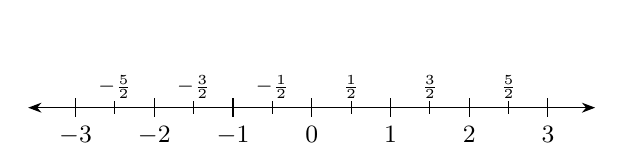
\begin{tikzpicture}[>=Stealth]
  \draw[<->] (-3.6,0) -- (3.6,0);
  \foreach \x/\l in {-3/-3,-2/-2,-1/-1,0/0,1/1,2/2,3/3}{
    \draw (\x,0.12) -- (\x,-0.12) node[below] {\small$\l$};
  }
  \foreach \x/\l in {-2.5/-\frac52,-1.5/-\frac32,-0.5/-\frac12,0.5/\frac12,1.5/\frac32,2.5/\frac52}{
    \draw (\x,0.08) -- (\x,-0.08) node[above=2pt] {\scriptsize$\l$};
  }
\end{tikzpicture}
\end{center}

\subsubsection*{Place Value}

Each place in a number is worth ten times the place to its right. Left of the decimal point we have
\[\cdots\ \text{ten thousands (}10{,}000),\ \text{thousands (}1{,}000),\ \text{hundreds (}100),\ \text{tens (}10),\ \text{ones (}1)\]
and right of the decimal point we have
\[\text{tenths}\left(\tfrac1{10}\right),\ \text{hundredths}\left(\tfrac1{100}\right),\ \text{thousandths}\left(\tfrac1{1000}\right),\ \text{ten-thousandths}\left(\tfrac1{10{,}000}\right)\ \cdots\]

\begin{center}
\begin{tabular}{c|c|c|c|c|c|c|c|c}
10,000 & 1,000 & 100 & 10 & 1 & . & $\tfrac1{10}$ & $\tfrac1{100}$ & $\tfrac1{1000}$\\
\hline
1 & 0 & 0 & 0 & 0 & . & & &\\
 & 1 & 0 & 0 & 0 & . & & &\\
 & & 1 & 0 & 0 & . & & &\\
 & & & 1 & 0 & . & & &\\
 & & & & 1 & . & & &\\
 & & & & & . & 1 & &\\
 & & & & & . & 0 & 1 &\\
 & & & & & . & 0 & 0 & 1
\end{tabular}
\end{center}
\[0.1=\frac1{10}\qquad0.01=\frac1{100}\qquad0.001=\frac1{1000}\qquad0.0001=\frac1{10{,}000}\]

\exbox{2} Consider the number $12.3456$. \seesol{2}
\begin{enumerate}[label=\alph*.,itemsep=0pt]
  \item What number is in the ones place?
  \item What number is in the hundredths place?
  \item What number is in the tens place?
  \item What number is in the tenths place?
  \item What number is in the thousandths place?
  \item What number is in the ten-thousandths place?
  \item What number is in the hundreds place?
\end{enumerate}

\subsubsection*{Expanded Form}

$12.3456$ can be written as
\[10+2+\frac3{10}+\frac4{100}+\frac5{1000}+\frac6{10{,}000}\]

\exbox{3} Write each number in expanded form. \seesol{3}
\begin{center}
$a.\ 3{,}502.23$\qquad $b.\ 56.128$\qquad $c.\ 235.568$
\end{center}

To go the other way, write everything over the same denominator and add:
\[\begin{aligned}
  200+30+5+\frac5{10}+\frac6{100}+\frac8{1000}
  &=\frac{200{,}000+30{,}000+5{,}000+500+60+8}{1000}\\
  &=\frac{235{,}568}{1000}=235.568
\end{aligned}\]

\subsubsection*{Changing Between Decimals and Fractions}

\[4.5\to4\frac5{10}\to\frac{45}{10}\qquad\qquad\frac{3278}{100}\to32\frac{78}{100}\to32.78=32\frac{39}{50}\]
(We reduced $\frac{78}{100}=\frac{39}{50}$ by dividing the top and bottom by $2$.)

Changing a decimal to a fraction: the digits become the numerator, and the denominator is $10$, $100$, $1000$, \ldots, one zero for each digit after the decimal point.
\[1.2345=\frac{12345}{10000}\qquad\text{and}\qquad\frac{27198}{1000}=27.198\]

\exbox{4} Change each decimal to a fraction and reduce to lowest terms. \seesol{4}
\begin{center}
$a.\ 0.35$\qquad $b.\ 0.125$\qquad $c.\ 0.375$
\end{center}

\subsubsection*{Comparing Decimals}

\textbf{Which is bigger, $0.1$ or $0.01$?}
\[0.1=\frac1{10}=\frac{1\cdot10}{10\cdot10}=\frac{10}{100}\qquad0.01=\frac1{100}\]
Since $\dfrac{10}{100}>\dfrac1{100}$, we have $0.1>0.01$.

\textbf{Which is bigger, $4.25$ or $4.227$?}
\[4+\frac{25}{100}=\frac{4000}{1000}+\frac{250}{1000}=\frac{4250}{1000}\qquad4+\frac{227}{1000}=\frac{4227}{1000}\]
So $4.227<4.25$.

\begin{keybox}
To compare decimals, add zeros at the end of the shorter decimal so both have the same number of places, then compare as if there were no decimal points.
\end{keybox}

\begin{align*}
8.34\text{ and }8.348&\to8.340\text{ and }8.348\to8.340<8.348\\
-4.25\text{ and }-4.227&\to-4.250\text{ and }-4.227\to-4.250<-4.227\\
-7.86\text{ and }-7.85&\to-7.86<-7.85
\end{align*}
(On the number line a negative number farther from $0$ is smaller.)

%=====================================================================
\subsection{Addition and Subtraction with Decimals}

Suppose you are told to add $18.5$ and $1.25$. How would we do this?

When we add two numbers we align the ones place. For integers that is the right-most digits:
\[
  \begin{array}{r}15\\+\ 7\\\hline22\end{array}\qquad
  \begin{array}{r}9\\+\ 8\\\hline17\end{array}\qquad
  \begin{array}{r}1173\\92\\+\ 351\\\hline1616\end{array}
\]
For decimals the ones place is the digit to the left of the decimal point, so \textbf{we line up the decimal points}:
\[
  \begin{array}{r}18.5\\+\ 1.25\\\hline\end{array}\qquad
  \begin{array}{r}23.0\\+\ 9\ \ \\\hline\end{array}\qquad
  \begin{array}{r}47.93\\+\ 2.5\ \ \\\hline\end{array}
\]
Let's do our original problem using mixed notation:
\[
  18.5+1.25=18\frac5{10}+1\frac{25}{100}=18\frac{50}{100}+1\frac{25}{100}=19\frac{75}{100}\to19.75
\]

\textbf{Example.} Solve by first changing to mixed notation: $25.43+2.897+379.6$.
\[\begin{aligned}
  25\frac{43}{100}+2\frac{897}{1000}+379\frac6{10}
  &=25\frac{430}{1000}+2\frac{897}{1000}+379\frac{600}{1000}\\
  &=406\frac{1927}{1000}=407\frac{927}{1000}=407.927
\end{aligned}\]

\textbf{Example.} Add $8+0.002+3.1+0.04$. Fill in zeros so that every number has the same number of decimal places:
\[
  \begin{array}{r}8.000\\0.002\\3.100\\+\ 0.040\\\hline11.142\end{array}
\]

\textbf{Example.} Subtract $5.9-3.0814$.
\[
  \begin{array}{r}5.9000\\-\ 3.0814\\\hline2.8186\end{array}
\]

\textbf{Example.} Subtract $3.09$ from the sum of $9$ and $5.472$.
\[9+5.472=14.472\qquad\qquad14.472-3.090=11.382\]

\textbf{Examples with negatives.} $-4.75+(-2.25)=-(4.75+2.25)=-7.00$.

$3.42+(-6.89)=3.42-6.89=-(6.89-3.42)=-3.47$.

%=====================================================================
\subsection{Multiplication with Decimals}

Let's say you're shopping at a store and you see a sign that says ``half off label price.'' You find something you like with a label price of $\$46.80$. How much would you actually pay for it?
\[\frac{46.80}2\qquad\frac12=0.5\qquad46.80\times\frac12=46.80\times0.5=23.40\]

\textbf{Example.} $0.5\times0.3$
\[\frac5{10}\times\frac3{10}=\frac{15}{100}=0.15\]

\textbf{Example.} $0.05\times0.003$
\[\frac5{100}\times\frac3{1000}=\frac{15}{100{,}000}=0.00015\]

\textbf{Example.} $2.1\times0.07$
\[
  2\frac1{10}\times\frac7{100}=\left(\frac{20}{10}+\frac1{10}\right)\times\frac7{100}=\frac{21}{10}\times\frac7{100}=\frac{147}{1000}=0.147
\]

\begin{keybox}
\textbf{Rule for multiplying decimals.}\\
1. Multiply as you would if the decimal points weren't there.\\
2. Place the decimal point in the answer so that the number of digits to the right of the decimal point is the total of the number of digits to the right of the decimal points in the numbers being multiplied.
\end{keybox}

Why does this work? Take $0.a\times0.bc$:
\[\frac a{10}\times\frac{bc}{100}=\frac{a\cdot bc}{10\cdot100}=\frac{abc}{1000}\]
and the three digits after the decimal point come from $1+2=3$ digits.

\textbf{Example.} $3.05\times4.36$. Multiply $305\times436=132{,}980$. There are $2+2=4$ decimal places, so the answer is $13.2980=13.298$.

\textbf{Example.} $0.05\times1.37\times21.25$.\\
First $1.37\times0.05$: $137\times5=685$, four decimal places in total ($2+2$), so $0.0685$.\\
Then $21.25\times0.0685$: $2125\times685=1{,}455{,}625$ with $2+4=6$ decimal places, so the answer is $1.455625$.

\textbf{Example.} $0.05(4.2+0.03)=0.05(4.23)=0.2115$.

\textbf{Example.} $4.8+12(3.2)^2$. Exponent first: $(3.2)^2=10.24$. Then $12\times10.24=122.88$, and $4.8+122.88=127.68$.

\textbf{Example.} Multiply with negatives. $a.\ (-5)(3.4)=-17.0$\qquad $b.\ (-0.4)(-0.8)=0.32$

%=====================================================================
\subsection{Division with Decimals}

\textbf{Example.} $5974\div20$. Long division, adding a decimal point and a zero:
\[5974\div20=298.7\]
To check, $20\times298.7=5974$.

\textbf{Example.} $34.8\div4=8.7$.

\begin{keybox}
\textbf{Rule.} To divide a decimal by a whole number, we do the usual long division with the decimal point of the answer placed directly above the decimal point in the problem.
\end{keybox}

\textbf{Example.} $49.896\div27=1.848$.\qquad\textbf{Example.} $1138.9\div35=32.54$.\qquad\textbf{Example.} $370.4\div8=46.3$.\qquad\textbf{Example.} $35.56\div2=17.78$.

\subsubsection*{Dividing by a Decimal}

If the divisor is a decimal, we multiply the numerator and denominator by a power of $10$ to make it a whole number. This gives an \textbf{equivalent fraction} (for example $\frac42$ and $\frac{40}{20}$).

\textbf{Example.} What is the quotient of $31.35$ and the sum of $1.26$ and $2.54$?
\[
  31.35\div(1.26+2.54)=31.35\div3.80\qquad\frac{31.35\times10}{3.8\times10}=\frac{313.5}{38}=8.25
\]

\textbf{Example.} $(0.2+0.177+0.0008)\div0.25$. First $0.2+0.177+0.0008=0.3778$. Then
\[
  0.3778\div0.25=\frac{0.3778\times100}{0.25\times100}=\frac{37.78}{25}=1.5112
\]

\textbf{Example.} $3.125\div0.005=\dfrac{3125}{5}=625$.

\textbf{Example.} $17\div0.03=\dfrac{17\times100}{0.03\times100}=\dfrac{1700}3=566.666\ldots$

%=====================================================================
\subsection{Rounding Decimals}

\begin{keybox}
If the number to the right of the place we are rounding to is less than $5$ ($<5$) we leave the number in the place alone. If it is greater than or equal to $5$ ($\geq5$) we increase the number in the place we're rounding to by $1$.
\end{keybox}

\begin{center}
\begin{tabular}{r|c|c|c}
 & Hundredths & Tenths & Whole number\\
\hline
$24.785$ & $24.79$ & $24.8$ & $25$\\
$2.3914$ & $2.39$ & $2.4$ & $2$\\
$0.98243$ & $0.98$ & $1.0$ & $1$\\
$14.0942$ & $14.09$ & $14.1$ & $14$\\
$0.545$ & $0.55$ & $0.5$ & $1$
\end{tabular}
\end{center}

\textbf{Example.} Round $9{,}235.492$ to the nearest hundred: $9{,}200$.\\
\textbf{Example.} Round $0.00346$ to the nearest thousandth: $0.0035$.

%=====================================================================
\subsection{Fractions and Decimals}

To write a fraction as a decimal, divide the numerator by the denominator.

\textbf{Example.} Write $\dfrac34$ as a decimal. $3\div4=0.75$.

\textbf{Example.} $\dfrac7{12}$. Dividing $7.000000\div12$ gives $0.58333\ldots$ The $3$ repeats forever. We write
\[\frac7{12}\approx0.583\qquad\text{or}\qquad\frac7{12}=0.58\overline3\]
where $\approx$ means ``approximately equal to'' and the bar marks the repeating digit.

\textbf{Example.} $\dfrac3{11}=0.272727\ldots=0.\overline{27}$.

\textbf{Example.} $-15.89\div14=-1.135$.

\textbf{Example.} $31.76\div2.3=\dfrac{317.6}{23}=13.808695652\ldots$

\textbf{Example.} Convert $0.075$ to a fraction and reduce.
\[0.075=\frac{75}{1000}=\frac{3\cdot5\cdot5}{2\cdot2\cdot2\cdot5\cdot5\cdot5}=\frac3{40}\]

\textbf{Example.} Write $0.38$ in lowest terms: $\dfrac{38}{100}=\dfrac{19}{50}$.

\textbf{Example.} Simplify $\dfrac{19}{50}(1.32+0.48)$.

Add first: $\dfrac{19}{50}(1.80)$. Convert the fraction: $19\div50=0.38$. Then $0.38\times1.80=0.684$.

\textbf{Example.} Simplify $\dfrac12+(0.75)\dfrac25$ in two ways.

\emph{Using decimals.} $\frac12=0.5$ and $\frac25=0.4$, so $0.5+(0.75)(0.4)=0.5+0.3=0.8$.

\emph{Using fractions.} $0.75=\frac{75}{100}=\frac34$, so
\[\frac12+\frac34\cdot\frac25=\frac12+\frac6{20}=\frac{10}{20}+\frac6{20}=\frac{16}{20}=\frac{8}{10}=\frac45\]
and $\frac45=0.8$.

\textbf{Example.} Simplify $\left(\dfrac12\right)^3(2.4)+\left(\dfrac14\right)^2(3.2)$.
\begin{gather*}
  \left(\tfrac12\right)^3=\tfrac18=0.125\qquad\left(\tfrac14\right)^2=\tfrac1{16}=0.0625\\
  0.125(2.4)+0.0625(3.2)=0.3+0.2=0.5
\end{gather*}

%=====================================================================
\subsection{Percents, Decimals, and Fractions}

\begin{keybox}
\textbf{Percent} means ``per hundred'' and is written $\%$. So $42\%=\dfrac{42}{100}$.
\end{keybox}

\textbf{Example.} Write as a fraction: $a.\ 33\%$\quad $b.\ 6\%$\quad $c.\ 160\%$
\[\frac{33}{100}\qquad\qquad\frac6{100}=\frac3{50}\qquad\qquad\frac{160}{100}=\frac{16}{10}=\frac85=1\frac35\]

\subsubsection*{Percent to Decimal}
\[35.2\%=\frac{35.2}{100}=0.352\]

\begin{keybox}
\textbf{Rule.} To change a percent to a decimal, move the decimal point two places to the left.
\end{keybox}

\textbf{Example.} Write as a decimal: $a.\ 37\%$\quad $b.\ 68\%$\quad $c.\ 120\%$\quad $d.\ 0.8\%$
\[0.37\qquad0.68\qquad1.20\qquad0.008\]

\subsubsection*{Decimal to Percent}
To change a decimal to a percent, move the decimal point two places to the right.
\[a.\ 0.27=27\%\qquad b.\ 4.89=489\%\qquad c.\ 0.5=50\%\qquad d.\ 0.09=9\%\]

\subsubsection*{Fraction to Percent}
Change the fraction to a decimal, then to a percent.
\[\frac7{10}=0.7=70\%\qquad\frac38=0.375=37.5\%\qquad2\frac12=2.5=250\%\]
\[\frac5{12}=0.41\overline6\quad\text{Round: }\frac5{12}\approx0.417=41.7\%\approx42\%\]

%=====================================================================
\pagebreak
\subsection{Examples}

\solsec{1}
$a.\ \dfrac{10}3\to\dfrac33+\dfrac33+\dfrac33+\dfrac13=3\dfrac13$\\[4pt]
$b.\ \dfrac95\to\dfrac55+\dfrac45=1\dfrac45$\\[4pt]
$c.\ \dfrac{21}4\to5\dfrac14$ (since $5\cdot4=20$ and $21-20=1$)

\solsec{2}
$a.\ 2$\quad $b.\ 4$\ (it represents $\frac4{100}$)\quad $c.\ 1$\quad $d.\ 3$\quad $e.\ 5$\quad $f.\ 6$\quad $g.\ 0$ (none)

\solsec{3}
$a.\ 3{,}000+500+0+2+\dfrac2{10}+\dfrac3{100}$\\[4pt]
$b.\ 50+6+\dfrac1{10}+\dfrac2{100}+\dfrac8{1000}$\\[4pt]
$c.\ 200+30+5+\dfrac5{10}+\dfrac6{100}+\dfrac8{1000}$

\solsec{4}
$a.\ 0.35=\dfrac{35}{100}=\dfrac{5\cdot7}{2\cdot2\cdot5\cdot5}=\dfrac7{20}$\\[4pt]
$b.\ 0.125=\dfrac{125}{1000}=\dfrac{5\cdot5\cdot5}{2\cdot2\cdot2\cdot5\cdot5\cdot5}=\dfrac18$\\[4pt]
$c.\ 0.375=\dfrac{375}{1000}=\dfrac{5\cdot5\cdot3\cdot5}{2\cdot5\cdot2\cdot5\cdot2\cdot5}=\dfrac3{2\cdot2\cdot2}=\dfrac38$
\part{Introduction to Algebra}

\clearpage
\def\chp{vars}
\source{Prealgebra}
\section{Introduction to Variables}
You already use algebra every day. You might figure out how much to tip a server, calculate the change you should get when you pay for something, or compare batting averages. In this section we explore the words used to describe algebra.

\subsection{Variables and Constants}

Greg and Alex have the same birthday but were born in different years. This year Greg is $20$ and Alex is $23$, so Alex is $3$ years older. When Greg was $12$, Alex was $15$. When Greg is $35$, Alex will be $38$. No matter what Greg's age is, Alex's age is always $3$ more.

In the language of algebra, we say that Greg's age and Alex's age are \textbf{variable}, and the $3$ is a \textbf{constant}. The ages change, or vary, but the $3$ years between them always stays the same.

In algebra, letters of the alphabet are used to represent variables. If we call Greg's age $g$, then Alex's age is $g+3$.

\begin{center}
\begin{tabular}{c|c}
Greg's age & Alex's age\\\hline
$12$ & $15$\\
$20$ & $23$\\
$35$ & $38$\\
$g$ & $g+3$
\end{tabular}
\end{center}

\begin{keybox}
A \textbf{variable} is a letter that represents a number or quantity whose value may change.\\
A \textbf{constant} is a number whose value always stays the same.
\end{keybox}

Letters often used for variables are $x$, $y$, $a$, $b$ and $c$.

\exbox{1} Identify the variable and the constant in each expression. \seesol{1}
\begin{center}
$a.\ y+7\qquad\qquad b.\ 32-x$
\end{center}

\pagebreak
\subsection{Examples}

\solsec{1}
$a.$ $y$ is the variable and $7$ is the constant.\\
$b.$ $x$ is the variable and $32$ is the constant.
\clearpage
\def\chp{lin1}
\lfoot{}
\section{Linear Equations in One Variable}
%=====================================================================
Examples of linear equations in one variable:
\[3x+2=17\qquad\qquad7a+4=3a-2\]

\begin{keybox}
\textbf{Steps to solve a linear equation in one variable}\\
\textbf{Step 1.} Simplify each side of the equation as much as possible.\\
\textbf{Step 2.} Use the addition property of equality to get all the variable terms on one side and the constants on the other, then combine like terms.\\
\textbf{Step 3.} Use the multiplication property to get the variable by itself.\\
\textbf{Step 4.} Check your solution.
\end{keybox}

\textbf{Example.} Solve $3(x+2)=-9$.
\begin{align*}
  \text{Step 1:}\quad 3x+6&=-9\\
  \text{Step 2:}\quad 3x+6-6&=-9-6\\
  3x&=-15\\
  \text{Step 3:}\quad\frac{3x}3&=\frac{-15}3\\
  x&=-5\\
  \text{Step 4:}\quad 3(-5+2)=3(-3)&=-9\ \checkmark
\end{align*}

\textbf{Example.} Solve $\dfrac x2+\dfrac x6=8$. Factor out $x$ using the distributive property:
\begin{align*}
  x\cdot\frac12+x\cdot\frac16&=8\\
  x\left(\frac12+\frac16\right)&=8\\
  x\left(\frac36+\frac16\right)&=8\\
  x\cdot\frac46=x\cdot\frac23&=8
\end{align*}
\[x=8\cdot\frac32=\frac{2\cdot2\cdot2\cdot3}{2}=4\cdot3=12\]

%=====================================================================
\subsection{Evaluating Variable Expressions}

\subsubsection*{The Distributive Property}

\[5(x+3)=5x+5\cdot3=5x+15\]
\[-\frac14(8x+12)=-\frac{8x}4-\frac{12}4=-2x-3\]

\subsubsection*{Combining Like Terms}

\textbf{Example.} Simplify $\dfrac23x-2+\dfrac13x+7$. Group like terms:
\[\frac23x+\frac13x-2+7=\left(\frac23+\frac13\right)x+5=\frac33x+5=x+5\]

\textbf{Example.} $-2(3y+4)+5=-6y-8+5=-6y-3$.

\textbf{Example.} $2(3x+1)+4(2x-5)=6x+2+8x-20=6x+8x+2-20=14x-18$.

\subsubsection*{Algebraic Expressions}

An \textbf{algebraic expression} such as $3x+5$ has a value once we know what $x$ is. We replace $x$ with the number and compute.
\[\text{For }x=2:\ 3(2)+5=6+5=11\qquad\qquad\text{For }x=10:\ 3(10)+5=30+5=35\]

\textbf{Example.} Evaluate $-\dfrac14x+5$ when $x=-8$.
\[-\frac14(-8)+5=\frac84+5=2+5=7\]

%=====================================================================
\subsection{The Addition Property of Equality}

Two angles $A$ and $B$ that together make a right angle satisfy
\[A+B=90^\circ.\]
So if $A=30^\circ$ then $30^\circ+B=90^\circ$, and $B=90^\circ-30^\circ=60^\circ$.

\begin{center}
\begin{tikzpicture}[>=Stealth]
  \draw[->] (0,0) -- (0,2.6);
  \draw[->] (0,0) -- (3.6,0);
  \draw[->] (0,0) -- (3.2,1.85);
  \draw (0,0.3) -- (0.3,0.3) -- (0.3,0);
  \draw (0.9,0) arc (0:30:0.9) node[midway,right] {\scriptsize$B$};
  \draw (0,0.6) arc (90:30:0.6) node[midway,above right] {\scriptsize$A$};
\end{tikzpicture}
\end{center}

\begin{keybox}
A \textbf{solution} for an equation is a number that makes the statement true.
\end{keybox}

\textbf{Example.} For the equation $x+3=7$, what value of $x$ makes the statement true? $x+3=7\to x=7-3\to x=4$. The solution is $4$.

\textbf{Example.} Is $a=-2$ the solution to the equation $7a+4=3a-2$?
\[7(-2)+4=3(-2)-2\quad\to\quad-14+4=-6-2\quad\to\quad-10=-8\]
This is not true, so \textbf{No}, $a=-2$ is not a solution.

To remove a number that is being added in an equation, we must subtract it, and to keep the equation balanced it must be done to both sides. Note: subtracting a negative number is the same as adding the opposite.

\begin{keybox}
\textbf{Addition Property.} If $A=B$ then $A+C=B+C$.\\[4pt]
If $A+B=C$, to get $B$ to the other side:
\[A+B-B=C-B\quad\Rightarrow\quad A=C-B\]
If $A-B=C$:
\[A-B+B=C+B\quad\Rightarrow\quad A=C+B\]
\end{keybox}

\textbf{Example.} Solve for $x$.\\
$a.\ x+4=-2$: subtract $4$ from both sides, $x=-2-4=-6$. Check: $-6+4=-2\ \checkmark$\\[4pt]
$b.\ 3x-2-2x=4-9$: combine, $(3x-2x)-2=-5$, so $x-2=-5$ and $x=-5+2=-3$.\\
Check: $3(-3)-2-2(-3)=-9-2+6=-5=4-9\ \checkmark$\\[4pt]
$c.\ x-\dfrac34=\dfrac58$: $x=\dfrac58+\dfrac{3\cdot2}{4\cdot2}=\dfrac58+\dfrac68=\dfrac{11}8$.\\
Check: $\dfrac{11}8-\dfrac34=\dfrac{11}8-\dfrac68=\dfrac58\ \checkmark$

\subsubsection*{Angles}

A right angle is $90^\circ$. A straight angle is $180^\circ$.

\textbf{Example.} Two angles make a right angle. One is $30^\circ$ and the other is $x$: $30^\circ+x=90^\circ$ so $x=60^\circ$.\\
\textbf{Example.} Two angles make a straight angle. One is $45^\circ$: $45^\circ+x=180^\circ$ so $x=135^\circ$.\\
\textbf{Example.} One angle is $57^\circ$ on a straight line: $x=180^\circ-57^\circ=123^\circ$.

\subsubsection*{Solving with Both Properties}

\textbf{Example.} $4a+5=2a-7$.
\begin{align*}
  4a+5-5&=2a-7-5\\
  4a&=2a-12\\
  4a-2a&=2a-12-2a\\
  2a&=-12\\
  a&=-6
\end{align*}
Check: $4(-6)+5=-24+5=-19$ and $2(-6)-7=-12-7=-19\ \checkmark$

\textbf{Example.} $2(x-4)+5=-11$.
\[2x-8+5=-11\ \to\ 2x-3=-11\ \to\ 2x=-8\ \to\ x=-4\]
Check: $2(-4-4)+5=2(-8)+5=-16+5=-11\ \checkmark$

\textbf{Example.} $5(2x-4)+3=4x-5$.
\begin{gather*}10x-20+3=4x-5\ \to\ 10x-17=4x-5\\ 10x-4x=-5+17\ \to\ 6x=12\ \to\ x=2\end{gather*}

%=====================================================================
\subsection{The Multiplication Property of Equality}

\begin{keybox}
\textbf{Multiplication Property.} When $C\neq0$: if $A=B$ then $AC=BC$.
\end{keybox}

Remember \textbf{reciprocals}: the number we multiply by to get $1$. The reciprocal of $\dfrac ab$ is $\dfrac ba$.

\textbf{Example.} Solve $\dfrac12x=3$. Multiply both sides by $2$:
\[2\cdot\frac12x=3\cdot2\ \to\ 1x=6\ \to\ x=6\]

In general if $A\cdot\dfrac1B=C$ then $A\cdot\dfrac1B\cdot B=C\cdot B$, so $A=C\cdot B$. And if $A\cdot B=C$ then $A\cdot B\cdot\dfrac1B=C\cdot\dfrac1B$, so $A=\dfrac CB$.

\textbf{Example.} $4x=-20$:\quad $4x\cdot\dfrac14=-20\cdot\dfrac14\ \to\ x=-5$. Check: $4(-5)=-20\ \checkmark$

\textbf{Example.} $-3x+7=-5$:
\[-3x=-5-7=-12\ \to\ -3x\cdot\frac1{-3}=-12\cdot\frac1{-3}\ \to\ x=4\]
Check: $-3(4)+7=-12+7=-5\ \checkmark$

\textbf{Example.} $5x-8x+3=4-10$:
\[(5x-8x)+3=4-10\ \to\ -3x+3=-6\ \to\ -3x=-9\ \to\ x=\frac{-9}{-3}=3\]
Check: $5(3)-8(3)+3=15-24+3=-6=4-10\ \checkmark$

\subsubsection*{Equations with Fractions}

\textbf{Example.} $\dfrac13x+2=7$.
\[\frac13x=5\ \to\ x=5\cdot3=15\]
Check: $\dfrac13(15)+2=5+2=7\ \checkmark$

\textbf{Example.} $-\dfrac45x=\dfrac8{15}$. Multiply by the reciprocal $-\dfrac54$:
\[x=\frac8{15}\left(-\frac54\right)=-\frac{2\cdot4\cdot5}{3\cdot5\cdot4}=-\frac23\]
Check: $-\dfrac45\left(-\dfrac23\right)=\dfrac8{15}\ \checkmark$

\textbf{Example.} $2x+\dfrac12=\dfrac34$.
\[2x=\frac34-\frac{1\cdot2}{2\cdot2}=\frac34-\frac24=\frac14\ \to\ x=\frac14\cdot\frac12=\frac18\]

\textbf{Example.} $\dfrac3x+2=\dfrac12$.
\[\frac3x=\frac12-\frac{2\cdot2}{1\cdot2}=\frac12-\frac42=-\frac32\]
If $\dfrac3x=-\dfrac32$, then taking reciprocals, $\dfrac x3=-\dfrac23$, so $x=-\dfrac23\cdot3=-2$.

%=====================================================================
\subsection{Equations Containing Decimals}

\textbf{Example.} $x-3.5=8.7$: $x=8.7+3.5=12.2$.

\textbf{Example.} $4y=-3.32$: $y=\dfrac{-3.32}4=-0.83$.

\textbf{Example.} $\dfrac12x-2.59=3.81$.
\[\frac12x=3.81+2.59=6.40\ \to\ x=2\cdot6.40=12.8\]

\textbf{Example.} $7a+0.61=-5a-0.89$.
\[7a+5a=-0.89-0.61\ \to\ 12a=-1.50\ \to\ a=\frac{-1.50}{12}=-0.125\]
(One way to see this: $-\dfrac{150}{100}\cdot\dfrac1{12}=-\dfrac32\cdot\dfrac1{12}=-\dfrac3{24}=-\dfrac18=-0.125$.)

\textbf{Example.} $7a+0.61=5a-0.89$.
\[2a=-0.89-0.61=-1.50\ \to\ a=-0.75\]

\textbf{Example.} $1.18x+0.24=0.84x-0.78$.
\[1.18x-0.84x=-0.78-0.24\ \to\ 0.34x=-1.02\ \to\ x=\frac{-1.02}{0.34}=-3\]

%=====================================================================
\subsection{Applications}

\textbf{Example.} The sum of a number and $2$ is $8$. Find the number.
\[x+2=8\ \to\ x=8-2=6\]
The sum of $6$ and $2$ is $8$.

\textbf{Example.} If $5$ is added to the sum of twice a number and three times the number the result is $25$. Find the number.
\[5+(2x+3x)=25\ \to\ 5+5x=25\ \to\ 5x=20\ \to\ x=4\]
Check: $5+2(4)+3(4)=5+8+12=25\ \checkmark$

\textbf{Example.} The length of a rectangle is three times the width. The perimeter is $72$ cm. Find the width and length.

\begin{center}
\begin{tikzpicture}
  \draw (0,0) rectangle (4,1.3);
  \node[below] at (2,0) {$l$};
  \node[right] at (4,0.65) {$w$};
\end{tikzpicture}
\end{center}
\[l=3w\qquad P=l+l+w+w=2l+2w=72\]
\[2(3w)+2w=72\ \to\ 6w+2w=72\ \to\ 8w=72\ \to\ w=9\]
So the width is $9$ cm and the length is $l=3\cdot9=27$ cm. Check: $27+27+9+9=72\ \checkmark$

\textbf{Example.} JoAnn is $22$ years older than her daughter Stacey. In six years the sum of their ages will be $42$. How old are they now?

Let $J$ be JoAnn's age and $S$ be Stacey's age. $J=22+S$. In six years $(J+6)+(S+6)=42$.
\begin{align*}
  (22+S)+6+S+6&=42\\
  34+2S&=42\\
  2S&=8\\
  S&=4
\end{align*}
Stacey is $4$ and JoAnn is $J=22+4=26$.

\textbf{Example.} A car rental company charges $\$11$ per day and $16$ cents per mile for their cars. If a car were rented for $1$ day and the charge was $\$25.40$, how many miles was the car driven?
\[11\cdot1+0.16m=25.40\ \to\ 0.16m=14.40\ \to\ m=\frac{14.40}{0.16}=90\]
The car was driven $90$ miles.

%=====================================================================
\subsection{Evaluating Formulas}

\[F=\frac95C+32\]
is the conversion between Fahrenheit and Celsius. A \textbf{formula} is an equation that contains more than one variable. Here $F$ and $C$ are both variables.

\textbf{Example.} The perimeter of a rectangle is $2w+2l$. The perimeter of a livestock pen is $40$ ft. If the width is $6$ ft, what is the length?
\[2(6)+2l=40\ \to\ 12+2l=40\ \to\ 2l=28\ \to\ l=\frac{28}2=14\text{ ft}\]

\textbf{Example.} $C=\dfrac59(F-32)$. Find $C$ when $F$ is $95^\circ$.
\[C=\frac59(95-32)=\frac59(63)=\frac{5\cdot3\cdot3\cdot7}{3\cdot3}=5\cdot7=35\]

\textbf{Example.} $y=2x+6$. Find $y$ when $x=-2$: $y=2(-2)+6=-4+6=2$.

\textbf{Example.} $2x+3y=4$. Find $y$ when $x=3$.
\[2(3)+3y=4\ \to\ 6+3y=4\ \to\ 3y=-2\ \to\ y=-\frac23\]
\clearpage
\def\chp{ineq}
\source{Elementary Algebra}
\section{Solving Linear Inequalities}
\subsection{Graph Inequalities on the Number Line}

Recall that a \textbf{solution} of an equation is a value of the variable that makes a true statement when substituted into the equation. What about the solution of an inequality? What number would make $x>3$ true? $x$ could be $4$, but also $5$, $20$, or even $3.001$. Any number greater than $3$ is a solution.

We show the solutions of $x>3$ on the number line by shading all the numbers to the right of $3$. Because $3$ itself is not a solution, we put an \textbf{open parenthesis} at $3$.

\begin{center}
$x>3$\qquad\ineqline{-5}{5}{3}{1}{}
\end{center}

For $x\geq3$ we need to show that $3$ \emph{is} a solution too, so we put a \textbf{bracket} at $3$.

\begin{center}
$x\geq3$\qquad\ineqline{-5}{5}{3}{2}{}
\end{center}

\begin{keybox}
The parenthesis $($ shows that the endpoint of the inequality is \textbf{not} included. The bracket $[$ shows that the endpoint \textbf{is} included.
\end{keybox}

\exbox{1} Graph on the number line. \seesol{1}
\begin{center}
$a.\ x\leq1\qquad\qquad b.\ x<5\qquad\qquad c.\ x>-1$
\end{center}

\subsubsection*{Interval Notation}

We can also write inequalities in \textbf{interval notation}. The inequality $x>3$ means all numbers greater than $3$. There is no upper end, so we write $(3,\infty)$. The symbol $\infty$ is read ``infinity''; it is not an actual number. The inequality $x\leq1$ has no lower end, so we write $(-\infty,1]$, where $-\infty$ is read ``negative infinity''.

\begin{keybox}
The parenthesis or bracket in interval notation matches the symbol at the endpoint of the arrow.
\begin{center}
\renewcommand{\arraystretch}{1.3}
\begin{tabular}{c|c|c|c}
$x>a$ & $x\geq a$ & $x<a$ & $x\leq a$\\\hline
$(a,\infty)$ & $[a,\infty)$ & $(-\infty,a)$ & $(-\infty,a]$\\
parenthesis & bracket & parenthesis & bracket
\end{tabular}
\end{center}
Infinity always gets a parenthesis, since it is not a number we can reach.
\end{keybox}

\exbox{2} Graph on the number line and write in interval notation. \seesol{2}
\begin{center}
$a.\ x\geq-3\qquad\qquad b.\ x<2.5\qquad\qquad c.\ x\leq-\dfrac35$
\end{center}

%=====================================================================
\subsection{The Addition and Subtraction Properties of Inequality}

The Subtraction and Addition Properties of Equality say that if two quantities are equal, adding or subtracting the same amount from both gives equal results. Similar properties hold for inequalities. For example, $-4<2$. If we subtract $5$ from both sides we get $-9$ and $-3$, and $-9<-3$. The inequality sign stayed the same.

\begin{keybox}
\textbf{Properties of Inequality.} For any numbers $a$, $b$ and $c$:
\begin{center}
\begin{tabular}{l@{\qquad\qquad}l}
\textbf{Subtraction Property} & \textbf{Addition Property}\\
if $a<b$ then $a-c<b-c$ & if $a<b$ then $a+c<b+c$\\
if $a>b$ then $a-c>b-c$ & if $a>b$ then $a+c>b+c$
\end{tabular}
\end{center}
\end{keybox}

We use these properties to solve inequalities, taking the same steps we used to solve equations. For $x+5>9$:
\[x+5>9\ \to\ x+5-5>9-5\ \to\ x>4\]
Any number greater than $4$ is a solution.

\exbox{3} Solve $x+5\leq6$, graph the solution and write it in interval notation. \seesol{3}

\exbox{4} Solve $x-2>1$, graph the solution and write it in interval notation. \seesol{4}

\exbox{5} Solve $n-\dfrac12\leq\dfrac58$, graph the solution and write it in interval notation. \seesol{5}

%=====================================================================
\subsection{The Division and Multiplication Properties of Inequality}

The Division and Multiplication Properties of Equality say that if two quantities are equal, dividing or multiplying both by the same amount (not dividing by $0$) gives equal results. What happens to an inequality?

Start with $10<15$. If we divide both sides by $5$ we get $2<3$. If we multiply both sides by $5$ we get $50<75$. The sign stayed the same.

Now what if we divide or multiply by a \textbf{negative} number? Dividing $10<15$ by $-5$ gives $-2$ and $-3$, and $-2>-3$. Multiplying both sides by $-5$ gives $-50$ and $-75$, and $-50>-75$. \textbf{The inequality sign reversed.}

\begin{keybox}
\textbf{Division and Multiplication Properties of Inequality.} For any real numbers $a$, $b$, $c$:
\begin{align*}
\text{if }a<b\text{ and }c>0,&\text{ then }\frac ac<\frac bc\text{ and }ac<bc\\
\text{if }a>b\text{ and }c>0,&\text{ then }\frac ac>\frac bc\text{ and }ac>bc\\
\text{if }a<b\text{ and }c<0,&\text{ then }\frac ac>\frac bc\text{ and }ac>bc\\
\text{if }a>b\text{ and }c<0,&\text{ then }\frac ac<\frac bc\text{ and }ac<bc
\end{align*}
When we divide or multiply an inequality by a \textbf{positive} number, the inequality stays the same.\\
When we divide or multiply an inequality by a \textbf{negative} number, the inequality \textbf{reverses}.
\end{keybox}

Sometimes the variable ends up on the right. We can rewrite the inequality in reverse to put the variable on the left: $x>a$ has the same meaning as $a<x$. (If Xavier is taller than Alex, then Alex is shorter than Xavier.)

\exbox{6} Solve $7y<42$, graph the solution and write it in interval notation. \seesol{6}

\exbox{7} Solve $-10a\geq50$, graph the solution and write it in interval notation. \seesol{7}

\exbox{8} Solve $-20<\dfrac45u$, graph the solution and write it in interval notation. \seesol{8}

\exbox{9} Solve $\dfrac t{-2}\geq8$, graph the solution and write it in interval notation. \seesol{9}

%=====================================================================
\subsection{Inequalities That Require Simplification}

Most inequalities take more than one step. We follow the same steps we used to solve linear equations, but we pay close attention when multiplying or dividing by a negative number.

\exbox{10} Solve $4m\leq9m+17$, graph the solution and write it in interval notation. \seesol{10}

\exbox{11} Solve $8p+3(p-12)>7p-28$, graph the solution and write it in interval notation. \seesol{11}

Just like some equations are identities and some are contradictions, inequalities may be too. We recognize these when only constants are left as we solve. If the result is a \textbf{true} statement we have an \textbf{identity} (the solution is all real numbers). If the result is a \textbf{false} statement we have a \textbf{contradiction} (there is no solution).

\exbox{12} Solve $8x-2(5-x)<4(x+9)+6x$, graph the solution and write it in interval notation. \seesol{12}

\exbox{13} Solve $\dfrac13a-\dfrac18a>\dfrac5{24}a+\dfrac34$, graph the solution and write it in interval notation. \seesol{13}

%=====================================================================
\pagebreak
\subsection{Examples}

\solsec{1}
$a.$ $x\leq1$ means all numbers less than or equal to $1$. Shade to the left of $1$ and put a bracket at $1$.
\begin{center}\ineqline{-5}{5}{1}{4}{}\end{center}
$b.$ $x<5$ means all numbers less than $5$. Shade to the left of $5$ and put a parenthesis at $5$.
\begin{center}\ineqline{-5}{5}{5}{3}{}\end{center}
$c.$ $x>-1$ means all numbers greater than $-1$. Shade to the right of $-1$ and put a parenthesis at $-1$.
\begin{center}\ineqline{-5}{5}{-1}{1}{}\end{center}

\solsec{2}
$a.$ $x\geq-3$: shade right of $-3$ with a bracket. Interval notation: $[-3,\infty)$.
\begin{center}\ineqline{-5}{5}{-3}{2}{}\end{center}
$b.$ $x<2.5$: shade left of $2.5$ with a parenthesis. Interval notation: $(-\infty,2.5)$.
\begin{center}\ineqline{-5}{5}{2.5}{3}{2.5}\end{center}
$c.$ $x\leq-\frac35$: shade left of $-\frac35$ with a bracket. Interval notation: $\left(-\infty,-\frac35\right]$.
\begin{center}\ineqline{-5}{5}{-0.6}{4}{-\frac35}\end{center}

\solsec{3}
\begin{align*}
x+5&\leq6\\
x+5-5&\leq6-5&&\text{subtract $5$ from both sides}\\
x&\leq1
\end{align*}
Interval notation: $(-\infty,1]$.
\begin{center}\ineqline{-5}{5}{1}{4}{}\end{center}

\solsec{4}
\begin{align*}
x-2&>1\\
x-2+2&>1+2&&\text{add $2$ to both sides}\\
x&>3
\end{align*}
Interval notation: $(3,\infty)$.
\begin{center}\ineqline{-5}{5}{3}{1}{}\end{center}

\solsec{5}
\begin{align*}
n-\frac12&\leq\frac58\\
n-\frac12+\frac12&\leq\frac58+\frac12&&\text{add $\tfrac12$ to both sides}\\
n&\leq\frac58+\frac48=\frac98
\end{align*}
Interval notation: $\left(-\infty,\frac98\right]$.
\begin{center}\ineqline{0}{3}{1.125}{4}{\frac98}\end{center}

\solsec{6}
\begin{align*}
7y&<42\\
\frac{7y}7&<\frac{42}7&&\text{divide by $7$; since $7>0$ the sign stays}\\
y&<6
\end{align*}
Interval notation: $(-\infty,6)$.
\begin{center}\ineqline{3}{8}{6}{3}{}\end{center}

\solsec{7}
\begin{align*}
-10a&\geq50\\
\frac{-10a}{-10}&\leq\frac{50}{-10}&&\text{divide by $-10$; since $-10<0$ the sign reverses}\\
a&\leq-5
\end{align*}
Interval notation: $(-\infty,-5]$.
\begin{center}\ineqline{-8}{-3}{-5}{4}{}\end{center}

\solsec{8}
\begin{align*}
-20&<\frac45u\\
\frac54(-20)&<\frac54\left(\frac45u\right)&&\text{multiply by $\tfrac54$; since $\tfrac54>0$ the sign stays}\\
-25&<u\\
u&>-25&&\text{rewrite with the variable on the left}
\end{align*}
Interval notation: $(-25,\infty)$.
\begin{center}\ineqline{-27}{-22}{-25}{1}{}\end{center}

\solsec{9}
\begin{align*}
\frac t{-2}&\geq8\\
-2\left(\frac t{-2}\right)&\leq-2(8)&&\text{multiply by $-2$; since $-2<0$ the sign reverses}\\
t&\leq-16
\end{align*}
Interval notation: $(-\infty,-16]$.
\begin{center}\ineqline{-19}{-14}{-16}{4}{}\end{center}

\solsec{10}
\begin{align*}
4m&\leq9m+17\\
4m-9m&\leq9m+17-9m&&\text{subtract $9m$ to collect the variables on the left}\\
-5m&\leq17\\
\frac{-5m}{-5}&\geq\frac{17}{-5}&&\text{divide by $-5$ and reverse the inequality}\\
m&\geq-\frac{17}5
\end{align*}
Interval notation: $\left[-\frac{17}5,\infty\right)$.
\begin{center}\ineqline{-5}{-1}{-3.4}{2}{-\frac{17}5}\end{center}

\solsec{11}
\begin{align*}
8p+3(p-12)&>7p-28\\
8p+3p-36&>7p-28&&\text{distribute}\\
11p-36&>7p-28&&\text{combine like terms}\\
11p-36-7p&>7p-28-7p&&\text{subtract $7p$}\\
4p-36&>-28\\
4p-36+36&>-28+36&&\text{add $36$}\\
4p&>8\\
\frac{4p}4&>\frac84&&\text{divide by $4$; the sign stays}\\
p&>2
\end{align*}
Interval notation: $(2,\infty)$.
\begin{center}\ineqline{-1}{4}{2}{1}{}\end{center}

\solsec{12}
\begin{align*}
8x-2(5-x)&<4(x+9)+6x\\
8x-10+2x&<4x+36+6x&&\text{distribute}\\
10x-10&<10x+36&&\text{combine like terms}\\
10x-10-10x&<10x+36-10x&&\text{subtract $10x$}\\
-10&<36
\end{align*}
The $x$'s are gone and we have a true statement, so the inequality is an \textbf{identity}. The solution is all real numbers, $(-\infty,\infty)$.
\begin{center}\ineqline{-5}{5}{0}{5}{}\end{center}

\solsec{13}
\begin{align*}
\frac13a-\frac18a&>\frac5{24}a+\frac34\\
24\left(\frac13a-\frac18a\right)&>24\left(\frac5{24}a+\frac34\right)&&\text{multiply by the LCD, $24$}\\
8a-3a&>5a+18\\
5a&>5a+18&&\text{combine like terms}\\
5a-5a&>5a+18-5a&&\text{subtract $5a$}\\
0&>18
\end{align*}
The statement is false, so the inequality is a \textbf{contradiction}. There is \textbf{no solution}.
\part{Lines and Graphing}

\clearpage
\def\chp{lin2}
\lfoot{}
\section{Linear Equations in Two Variables}
%=====================================================================
\subsection{The Cartesian Plane and Paired Data}

\begin{keybox}
The \textbf{Cartesian plane} has two number lines: $x$ is the \textbf{horizontal axis} and $y$ is the \textbf{vertical axis}.
\end{keybox}

\textbf{Example.} The speed of a race car.

\begin{center}
\begin{tabular}{c|c}
time (seconds) & speed (mph)\\
\hline
0 & 0\\
1 & 72.7\\
2 & 129.9\\
3 & 162.8\\
4 & 192.2\\
5 & 212.4\\
6 & 228.1
\end{tabular}
\qquad
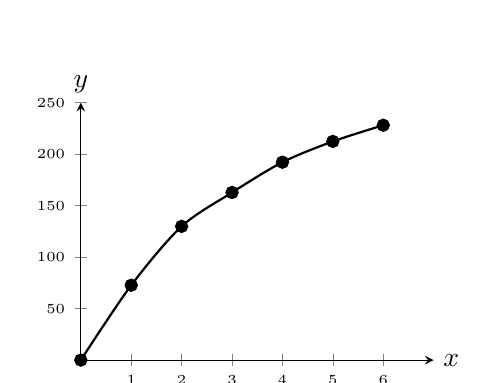
\begin{tikzpicture}
\begin{axis}[width=0.5\textwidth,height=0.4\textwidth,axis lines=left,
  xmin=0,xmax=7,ymin=0,ymax=250,xtick={1,...,6},ytick={50,100,...,250},
  xlabel={$x$},ylabel={$y$},tick label style={font=\tiny},
  every axis x label/.style={at={(ticklabel* cs:1.0)},anchor=west},
  every axis y label/.style={at={(ticklabel* cs:1.0)},anchor=south}]
\addplot[thick,mark=*,smooth] coordinates {(0,0)(1,72.7)(2,129.9)(3,162.8)(4,192.2)(5,212.4)(6,228.1)};
\end{axis}
\end{tikzpicture}
\end{center}

This is \textbf{paired data}: there is a speed associated with each time.

There is also a position and a value for paired data. For example if we have a list of odd numbers, each number has a position:
\[\{1,3,5,7,9,\ldots\}\qquad\text{first, second, third, fourth, fifth}\]

\begin{center}
\begin{tabular}{c|c}
\multicolumn{2}{c}{Odd numbers}\\
position & value\\\hline
1&1\\2&3\\3&5\\4&7\\5&9
\end{tabular}
\qquad\qquad
\begin{tabular}{c|c}
\multicolumn{2}{c}{Squares}\\
position & value\\\hline
1&1\\2&4\\3&9\\4&16\\5&25
\end{tabular}
\end{center}

\begin{center}
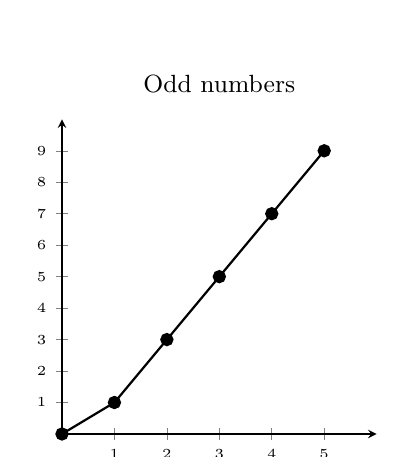
\begin{tikzpicture}
\begin{axis}[width=0.46\textwidth,height=0.46\textwidth,axis lines=left,
  xmin=0,xmax=6,ymin=0,ymax=10,xtick={1,...,5},ytick={1,...,9},
  tick label style={font=\tiny},title={Odd numbers},title style={font=\small}]
\addplot[thick,mark=*] coordinates {(0,0)(1,1)(2,3)(3,5)(4,7)(5,9)};
\end{axis}
\end{tikzpicture}
\hfill
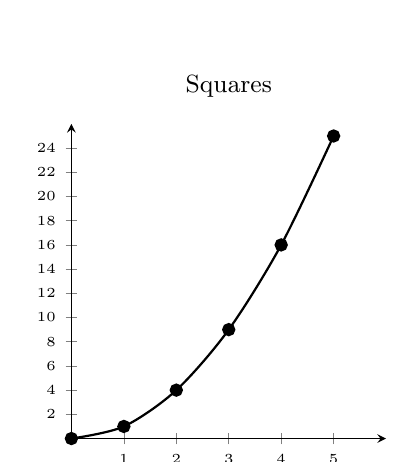
\begin{tikzpicture}
\begin{axis}[width=0.46\textwidth,height=0.46\textwidth,axis lines=left,
  xmin=0,xmax=6,ymin=0,ymax=26,xtick={1,...,5},ytick={2,4,...,24},
  tick label style={font=\tiny},title={Squares},title style={font=\small}]
\addplot[thick,mark=*,smooth] coordinates {(0,0)(1,1)(2,4)(3,9)(4,16)(5,25)};
\end{axis}
\end{tikzpicture}
\end{center}

\subsection{Ordered Pairs and Quadrants}

\begin{keybox}
An \textbf{ordered pair} $(x,y)$ names a point. The first number is the \textbf{$x$-coordinate} and the second is the \textbf{$y$-coordinate}.
\end{keybox}

To plot $(2,3)$:\quad 1. Start at the \textbf{origin}.\quad 2. Move across the $x$-axis.\quad 3. Move up or down the $y$-axis.

\begin{center}
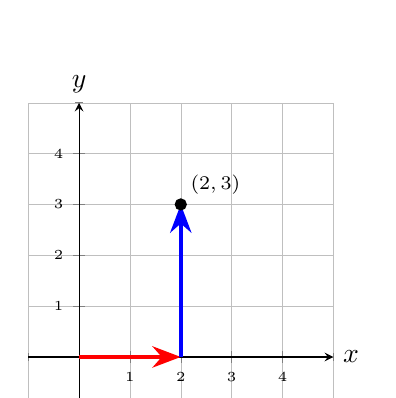
\begin{tikzpicture}
\begin{axis}[smallplane,width=0.45\textwidth,height=0.45\textwidth,xmin=-1,xmax=5,ymin=-1,ymax=5,
  xtick={1,...,4},ytick={1,...,4},minor xtick={-1,0,...,5},minor ytick={-1,0,...,5}]
\draw[ultra thick,red,-{Stealth}] (axis cs:0,0) -- (axis cs:2,0);
\draw[ultra thick,blue,-{Stealth}] (axis cs:2,0) -- (axis cs:2,3);
\addplot[only marks,mark=*] coordinates {(2,3)} node[above right] {\scriptsize$(2,3)$};
\end{axis}
\end{tikzpicture}
\end{center}

The axes divide the plane into four \textbf{quadrants}, labeled counterclockwise starting at the upper right.

\begin{center}
\begin{tikzpicture}[>=Stealth]
  \draw[<->] (-3.2,0) -- (3.2,0) node[right] {$x$};
  \draw[<->] (0,-3.2) -- (0,3.2) node[above] {$y$};
  \foreach \i in {-3,-2,-1,1,2,3}{
    \draw (\i,0.08) -- (\i,-0.08) node[below,font=\tiny] {$\i$};
    \draw (0.08,\i) -- (-0.08,\i) node[left,font=\tiny] {$\i$};
  }
  \node at (1.6,1.6) {Quadrant I};
  \node at (-1.6,1.6) {Quadrant II};
  \node at (-1.6,-1.6) {Quadrant III};
  \node at (1.6,-1.6) {Quadrant IV};
  \node[font=\scriptsize] at (0.55,-0.3) {origin};
\end{tikzpicture}
\end{center}

\exbox{1} Plot each point on a coordinate plane. \seesol{1}
\begin{center}
$a.\ (3,4)\ (3,-4)\ (-3,4)\ (-3,-4)$
\end{center}

\exbox{2} State the quadrant of each point, or say that it lies on an axis. \seesol{2}
\begin{center}
$a.\ (-1,3)\quad b.\ (2,5)\quad c.\ (0,0)\quad d.\ (0,-3)\quad e.\ (4,0)\quad f.\ (2,-3)$
\end{center}

\begin{center}
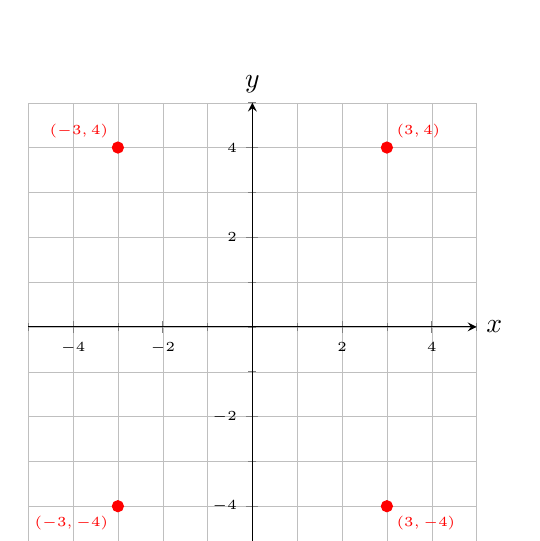
\begin{tikzpicture}
\begin{axis}[smallplane]
\addplot[only marks,mark=*,red] coordinates {(3,4)} node[above right,font=\tiny] {$(3,4)$};
\addplot[only marks,mark=*,red] coordinates {(3,-4)} node[below right,font=\tiny] {$(3,-4)$};
\addplot[only marks,mark=*,red] coordinates {(-3,4)} node[above left,font=\tiny] {$(-3,4)$};
\addplot[only marks,mark=*,red] coordinates {(-3,-4)} node[below left,font=\tiny] {$(-3,-4)$};
\end{axis}
\end{tikzpicture}
\end{center}

%=====================================================================
\subsection{Solutions to Linear Equations in Two Variables}

\begin{keybox}
In $y=-2x+3$, $x$ is the \textbf{independent variable} and $y$ is the \textbf{dependent variable}: the value of $y$ depends on the value of $x$.
\end{keybox}

To find possible solutions to an equation with two variables, get the variables on opposite sides of the equal sign, get the dependent variable by itself, then plug in a number for $x$ and find the corresponding $y$ value.

\textbf{Example.} $2x+3y=6$
\[2x=6-3y\quad\to\quad2x-6=-3y\quad\to\quad\frac{2x-6}{-3}=y\quad\to\quad y=-\frac23x+2\]

\begin{center}
\begin{tabular}{c|c}
$x$ & $y$\\\hline
0 & 2\\
1 & $\frac43$\\
2 & $\frac23$\\
3 & 0\\
4 & $-\frac23$\\
5 & $-\frac43$\\
6 & $-2$
\end{tabular}
\end{center}

\textbf{Example.} $2x+y=3$. Multiple answers could be true.
\begin{align*}
  x=2,\ y=-1:&\quad2(2)+(-1)=4+(-1)=3\ \checkmark\\
  x=0,\ y=3:&\quad2(0)+3=0+3=3\ \checkmark\\
  x=5,\ y=-7:&\quad2(5)+(-7)=10+(-7)=3\ \checkmark
\end{align*}
So $(2,-1)$, $(0,3)$ and $(5,-7)$ are all solutions. Solving for $y$ gives $y=-2x+3$ and we can make a table of as many solutions as we like:

\begin{center}
\begin{tabular}{c|c}
$x$ & $y$\\\hline
$-3$ & $9$\\
$-2$ & $7$\\
$-1$ & $5$\\
$0$ & $3$\\
$1$ & $1$\\
$2$ & $-1$\\
$3$ & $-3$\\
$4$ & $-5$\\
$5$ & $-7$
\end{tabular}
\end{center}

\textbf{Example.} $2x-5y=20$:
\[2x-20=5y\quad\to\quad y=\frac{2x-20}5=\frac25x-4\]
\begin{center}
\begin{tabular}{c|c|c|c|c|c|c|c|c|c|c|c}
$x$ & $-5$ & $-4$ & $-3$ & $-2$ & $-1$ & $0$ & $1$ & $2$ & $3$ & $4$ & $5$\\\hline
$y$ & $-6$ & $-\frac{28}5$ & $-\frac{26}5$ & $-\frac{24}5$ & $-\frac{22}5$ & $-4$ & $-\frac{18}5$ & $-\frac{16}5$ & $-\frac{14}5$ & $-\frac{12}5$ & $-2$
\end{tabular}
\end{center}

\textbf{Example.} $6=2(4x+1)-4y$:
\begin{align*}
  6+4y&=2(4x+1)\\
  6+4y&=8x+2\\
  4y&=8x+2-6\\
  4y&=8x-4\\
  y&=2x-1
\end{align*}

%=====================================================================
\subsection{Graphing Lines in the Plane}

To graph a line: solve for $y$, make a table of values, plot the points, and draw the line through them with arrows on the ends.

\exbox{3} Graph $y=2x-1$, $x+y=5$, $y=3x-1$ and $y=-\frac13x+2$. \seesol{3}

\begin{center}
\begin{tabular}{c|c}
\multicolumn{2}{c}{$y=2x-1$}\\
$x$ & $y$\\\hline
$-3$ & $-7$\\$-2$ & $-5$\\$-1$ & $-3$\\$0$ & $-1$\\$1$ & $1$\\$2$ & $3$\\$3$ & $5$
\end{tabular}\quad
\begin{tabular}{c|c}
\multicolumn{2}{c}{$x+y=5\to y=5-x$}\\
$x$ & $y$\\\hline
$-3$ & $8$\\$-2$ & $7$\\$-1$ & $6$\\$0$ & $5$\\$1$ & $4$\\$2$ & $3$\\$3$ & $2$
\end{tabular}\quad
\begin{tabular}{c|c}
\multicolumn{2}{c}{$y=3x-1$}\\
$x$ & $y$\\\hline
$-3$ & $-10$\\$-2$ & $-7$\\$-1$ & $-4$\\$0$ & $-1$\\$1$ & $2$\\$2$ & $5$\\$3$ & $8$
\end{tabular}\quad
\begin{tabular}{c|c}
\multicolumn{2}{c}{$y=-\frac13x+2$}\\
$x$ & $y$\\\hline
$-6$ & $4$\\$-3$ & $3$\\$0$ & $2$\\$3$ & $1$\\$6$ & $0$
\end{tabular}
\end{center}

\begin{center}
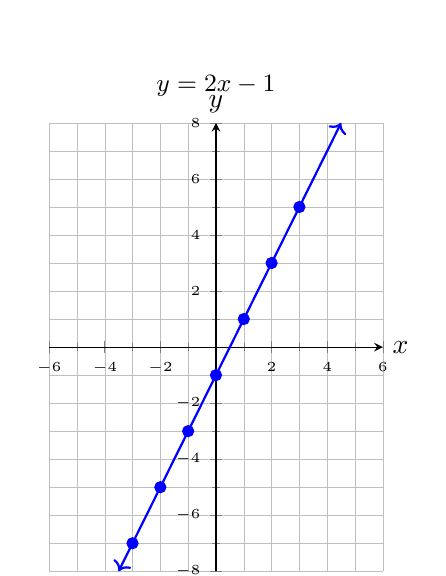
\begin{tikzpicture}
\begin{axis}[plane,title={$y=2x-1$}]
\addplot[thick,blue,<->,domain=-3.5:4.5,samples=2] {2*x-1};
\addplot[only marks,mark=*,blue] coordinates {(-3,-7)(-2,-5)(-1,-3)(0,-1)(1,1)(2,3)(3,5)};
\end{axis}
\end{tikzpicture}
\hfill
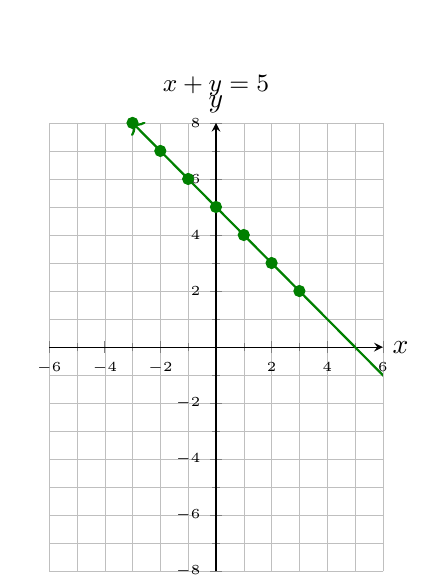
\begin{tikzpicture}
\begin{axis}[plane,title={$x+y=5$}]
\addplot[thick,green!50!black,<->,domain=-3:6.5,samples=2] {5-x};
\addplot[only marks,mark=*,green!50!black] coordinates {(-3,8)(-2,7)(-1,6)(0,5)(1,4)(2,3)(3,2)};
\end{axis}
\end{tikzpicture}

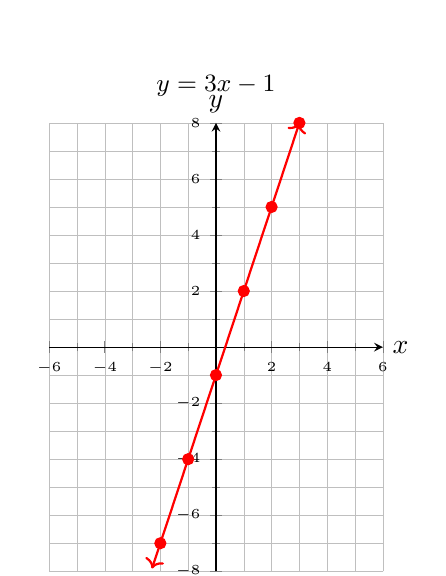
\begin{tikzpicture}
\begin{axis}[plane,title={$y=3x-1$}]
\addplot[thick,red,<->,domain=-2.3:3,samples=2] {3*x-1};
\addplot[only marks,mark=*,red] coordinates {(-2,-7)(-1,-4)(0,-1)(1,2)(2,5)(3,8)};
\end{axis}
\end{tikzpicture}
\hfill
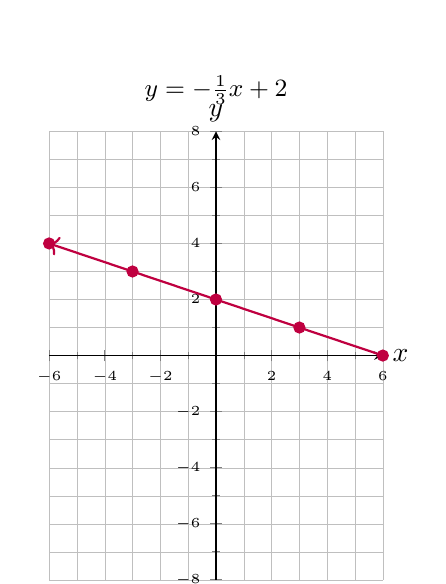
\begin{tikzpicture}
\begin{axis}[plane,title={$y=-\frac13x+2$}]
\addplot[thick,purple,<->,domain=-6:7,samples=2] {-x/3+2};
\addplot[only marks,mark=*,purple] coordinates {(-6,4)(-3,3)(0,2)(3,1)(6,0)};
\end{axis}
\end{tikzpicture}
\end{center}

\textbf{Example.} Graph $3x-2y=6$.
\[3x=6+2y\quad\to\quad3x-6=2y\quad\to\quad\frac{3x-6}2=y\quad\to\quad y=\frac32x-3\]
\begin{center}
\begin{tabular}{c|c|c|c|c|c|c|c|c|c}
$x$ & $-8$ & $-6$ & $-4$ & $-2$ & $0$ & $2$ & $4$ & $6$ & $8$\\\hline
$y$ & $-15$ & $-12$ & $-9$ & $-6$ & $-3$ & $0$ & $3$ & $6$ & $9$
\end{tabular}
\end{center}

\exbox{4} Graph each equation. \seesol{4}
\begin{center}
$a.\ y=\dfrac12x\qquad b.\ x=3\qquad c.\ y=-2$
\end{center}

\begin{center}
\begin{tabular}{c|c}
\multicolumn{2}{c}{$y=\frac12x$}\\$x$ & $y$\\\hline
$-6$ & $-3$\\$-4$ & $-2$\\$-2$ & $-1$\\$0$ & $0$\\$2$ & $1$\\$4$ & $2$\\$6$ & $3$
\end{tabular}\qquad
\begin{tabular}{c|c}
\multicolumn{2}{c}{$x=3$}\\$x$ & $y$\\\hline
$3$ & $1$\\$3$ & $2$\\$3$ & $3$
\end{tabular}\qquad
\begin{tabular}{c|c}
\multicolumn{2}{c}{$y=-2$}\\$x$ & $y$\\\hline
$0$ & $-2$\\$1$ & $-2$\\$2$ & $-2$\\$3$ & $-2$
\end{tabular}
\end{center}

\begin{center}
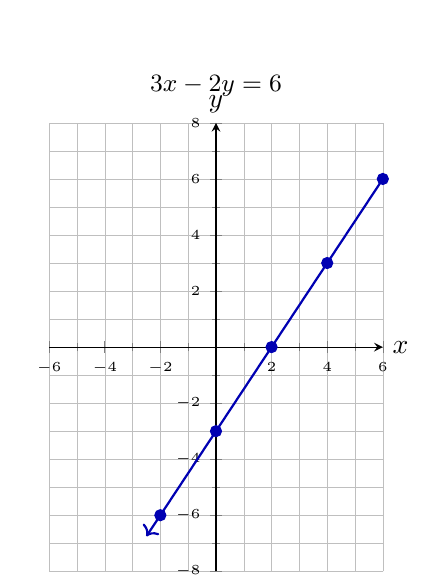
\begin{tikzpicture}
\begin{axis}[plane,title={$3x-2y=6$}]
\addplot[thick,blue!70!black,<->,domain=-2.5:6.7,samples=2] {1.5*x-3};
\addplot[only marks,mark=*,blue!70!black] coordinates {(-2,-6)(0,-3)(2,0)(4,3)(6,6)};
\end{axis}
\end{tikzpicture}
\hfill
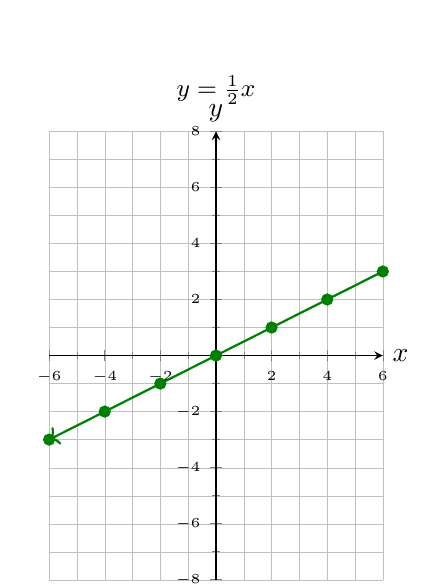
\begin{tikzpicture}
\begin{axis}[plane,title={$y=\frac12x$}]
\addplot[thick,green!50!black,<->,domain=-6:6.5,samples=2] {x/2};
\addplot[only marks,mark=*,green!50!black] coordinates {(-6,-3)(-4,-2)(-2,-1)(0,0)(2,1)(4,2)(6,3)};
\end{axis}
\end{tikzpicture}

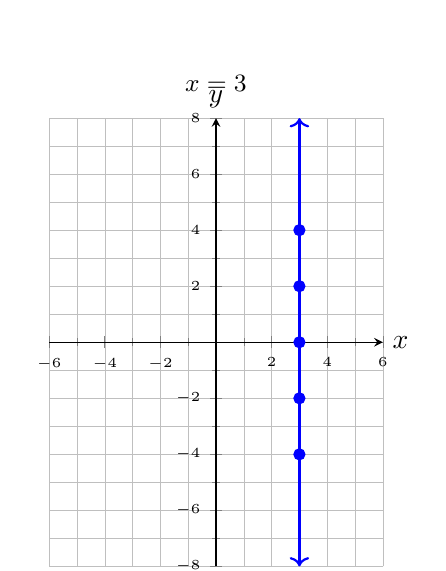
\begin{tikzpicture}
\begin{axis}[plane,title={$x=3$}]
\addplot[thick,blue,<->] coordinates {(3,-8)(3,8)};
\addplot[only marks,mark=*,blue] coordinates {(3,-4)(3,-2)(3,0)(3,2)(3,4)};
\end{axis}
\end{tikzpicture}
\hfill
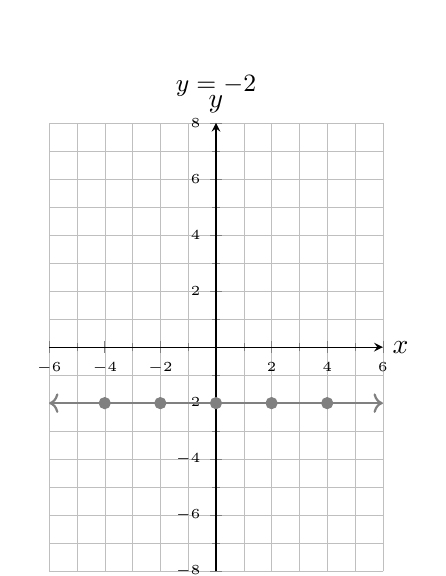
\begin{tikzpicture}
\begin{axis}[plane,title={$y=-2$}]
\addplot[thick,gray,<->] coordinates {(-6,-2)(6,-2)};
\addplot[only marks,mark=*,gray] coordinates {(-4,-2)(-2,-2)(0,-2)(2,-2)(4,-2)};
\end{axis}
\end{tikzpicture}
\end{center}

A vertical line $x=3$ has the same $x$-value for every point, and a horizontal line $y=-2$ has the same $y$-value for every point.

%=====================================================================
\subsection{Intercepts}

\begin{keybox}
An \textbf{intercept} is where the graphed line crosses an axis.\\[4pt]
The \textbf{$x$-intercept} is where the line crosses the $x$-axis, and where $y=0$.\\
The \textbf{$y$-intercept} is where the line crosses the $y$-axis, and where $x=0$.
\end{keybox}

\begin{center}
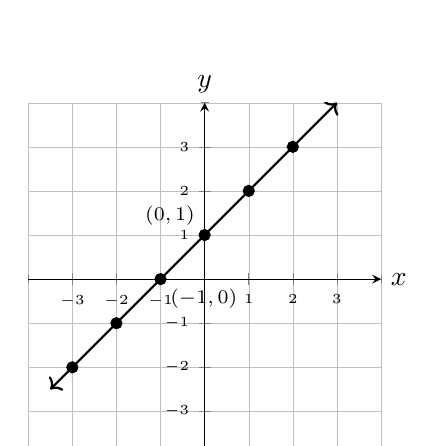
\begin{tikzpicture}
\begin{axis}[smallplane,width=0.5\textwidth,height=0.5\textwidth,xmin=-4,xmax=4,ymin=-4,ymax=4,
  xtick={-3,...,3},ytick={-3,...,3},minor xtick={-4,...,4},minor ytick={-4,...,4}]
\addplot[thick,<->,domain=-3.5:3,samples=2] {x+1};
\addplot[only marks,mark=*] coordinates {(-3,-2)(-2,-1)(-1,0)(0,1)(1,2)(2,3)};
\node[font=\scriptsize,above left] at (axis cs:0,1) {$(0,1)$};
\node[font=\scriptsize,below right] at (axis cs:-1,0) {$(-1,0)$};
\end{axis}
\end{tikzpicture}
\end{center}

Here the $y$-intercept is $(0,1)$ and the $x$-intercept is $(-1,0)$. So $y=1$ when $x=0$ and $x=-1$ when $y=0$.

\textbf{Example.} Find the intercepts of $3x-2y=6$. First solve for $2y$: $3x-6=2y$.

\emph{$x$-intercept} (set $y=0$): $3x-6=2(0)=0\ \to\ 3x=6\ \to\ x=\dfrac63=2$. The $x$-intercept is $(2,0)$.

\emph{$y$-intercept} (set $x=0$): $3(0)-6=2y\ \to\ -6=2y\ \to\ y=-3$. The $y$-intercept is $(0,-3)$.

\textbf{Example.} Find the intercepts of $-x+2y=4$. Then $2y=4+x$.

\emph{$x$-intercept:} $0=4+x\ \to\ x=-4$, so $(-4,0)$.\\
\emph{$y$-intercept:} $2y=4+0\ \to\ y=2$, so $(0,2)$.

\textbf{Example.} Find the intercepts of $-\dfrac13x+2=y$.

\emph{$x$-intercept:} $-\dfrac13x+2=0\ \to\ -\dfrac13x=-2\ \to\ x=-2\cdot(-3)=6$, so $(6,0)$.\\
\emph{$y$-intercept:} $0+2=y$, so $(0,2)$.

%=====================================================================
\pagebreak
\subsection{Examples}

\solsec{1}
Start at the origin, move across the $x$-axis by the first coordinate and up or down by the second. The four points are plotted in the graph above.

\solsec{2}
$a.\ (-1,3)$: Quadrant II\quad $b.\ (2,5)$: Quadrant I\quad $c.\ (0,0)$: the origin\quad $d.\ (0,-3)$: on the $y$-axis\quad $e.\ (4,0)$: on the $x$-axis\quad $f.\ (2,-3)$: Quadrant IV

\solsec{3}
See the four graphs above. Each line passes through every point in its table.

\solsec{4}
See the four graphs above. The graph of $3x-2y=6$ crosses the axes at $(2,0)$ and $(0,-3)$, the intercepts we found earlier.
\clearpage
\def\chp{slope}
\source{Prealgebra}
\section{Slope}
As we graph linear equations, we see that some lines slant up as they go from left to right and some slant down. Some lines are steep and some are flatter. What determines whether a line slants up or down, and whether its slant is steep or flat? The steepness of the slant of a line is called the \textbf{slope} of the line. Slope has many real-world uses: the pitch of a roof and the grade of a highway or wheelchair ramp are examples.

\subsection{Using a Geoboard to Model Slope}

Stretching a rubber band between two pegs on a geoboard gives a concrete way to model a line on a coordinate grid.

\begin{center}
\geoboard{\draw[orange,very thick] (0,0) -- (3,2); \draw[orange,very thick] (0,0) -- (0,2) -- (3,2);}
\end{center}

Here the band forms a line, and we stretched one part of it straight up from the left peg and over to the right to make a right triangle, with one side vertical and one side horizontal. The vertical leg goes up $2$ spaces, so the \textbf{rise} is $2$. The horizontal leg goes across $3$ spaces, so the \textbf{run} is $3$. (Count the \emph{spaces between} the pegs, not the pegs themselves.) The slope of this line is $\frac23$.

\begin{keybox}
The \textbf{slope} of a line is
\[m=\frac{\text{rise}}{\text{run}}.\]
The \textbf{rise} measures the vertical change and the \textbf{run} measures the horizontal change.
\end{keybox}

When we work with geoboards, start at a peg on the left and connect to a peg to the right, then stretch the band to form a right triangle. If we go up, the rise is positive. If we stretch down, the rise is \textbf{negative}. We always count the run from left to right, so the run is positive. Count the rise first, then the run.

\exbox{1} What is the slope of the line on the geoboard? \seesol{1}
\begin{center}
\geoboard{\draw[orange,very thick] (0,0) -- (4,3);}
\end{center}

\exbox{2} What is the slope of the line on the geoboard? \seesol{2}
\begin{center}
\geoboard{\draw[orange,very thick] (0,3) -- (3,2);}
\end{center}

Notice that in the first example the slope is positive and in the second the slope is negative. Reading from left to right, a line going up has \textbf{positive slope}, and a line going down has \textbf{negative slope}.

%=====================================================================
\subsection{Finding the Slope of a Line from its Graph}

To find the slope from a graph, we locate two points on the line, preferably with integer coordinates, start at the point on the left, and sketch a right triangle so we can count the rise and the run.

\begin{keybox}
\textbf{How to find the slope from a graph.}\\
\textbf{Step 1.} Locate two points on the line whose coordinates are integers.\\
\textbf{Step 2.} Starting with the point on the left, sketch a right triangle, going from the first point to the second point.\\
\textbf{Step 3.} Count the rise and the run on the legs of the triangle.\\
\textbf{Step 4.} Take the ratio of rise to run to find the slope, $m=\dfrac{\text{rise}}{\text{run}}$.
\end{keybox}

\exbox{3} Find the slope of the line through $(0,-3)$ and $(5,1)$ shown below. \seesol{3}
\begin{center}
\slopefig{xmin=-2,xmax=7,ymin=-5,ymax=3,xtick={-2,...,7},ytick={-5,...,3},title={$y=\frac45x-3$}}{0}{-3}{5}{1}{0.8*x-3}{-1}{6.5}
\end{center}

\exbox{4} Find the slope of the line through $(0,5)$ and $(3,3)$ shown below. \seesol{4}
\begin{center}
\slopefig{xmin=-1,xmax=9,ymin=-1,ymax=7,xtick={-1,...,9},ytick={-1,...,7},title={$y=-\frac23x+5$}}{0}{5}{3}{3}{-2*x/3+5}{-0.8}{8}
\end{center}

The slope of a line is the same no matter which two points we use. Using $(-3,7)$ and $(6,1)$ on the same line from Example 4 gives a rise of $-6$ and a run of $9$:
\[m=\frac{-6}9=-\frac23.\]
The slope of a line is constant!

\exbox{5} Find the slope of the line through $(2,3)$ and $(7,6)$ shown below. \seesol{5}
\begin{center}
\slopefig{xmin=-1,xmax=9,ymin=-1,ymax=8,xtick={-1,...,9},ytick={-1,...,8},title={}}{2}{3}{7}{6}{0.6*x+1.8}{-0.5}{8.5}
\end{center}

%=====================================================================
\subsection{Slope of Horizontal and Vertical Lines}

Horizontal lines have equations $y=b$ (all the $y$-coordinates are the same). Vertical lines have equations $x=a$ (all the $x$-coordinates are the same).

\textbf{Horizontal line $y=4$.} Use the points $(0,4)$ and $(3,4)$. The rise is $0$ and the run is $3$:
\[m=\frac03=0.\]

\textbf{Vertical line $x=3$.} Use the points $(3,0)$ and $(3,2)$. The rise is $2$ and the run is $0$:
\[m=\frac20\quad\text{which is undefined.}\]

\begin{keybox}
The slope of a \textbf{horizontal} line, $y=b$, is $0$.\\
The slope of a \textbf{vertical} line, $x=a$, is \textbf{undefined} (we cannot divide by $0$).
\end{keybox}

\exbox{6} Find the slope of each line. \seesol{6}
\begin{center}
$a.\ x=8\qquad\qquad b.\ y=-5$
\end{center}

\begin{keybox}
\textbf{Quick guide to the slopes of lines.}\\[4pt]
\begin{center}
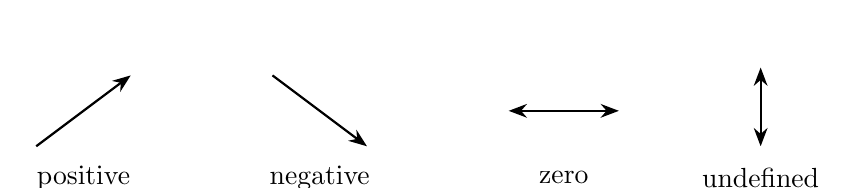
\begin{tikzpicture}[>=Stealth]
  \draw[->,thick] (0,0) -- (1.2,0.9); \node at (0.6,-0.4) {positive};
  \draw[->,thick] (3,0.9) -- (4.2,0); \node at (3.6,-0.4) {negative};
  \draw[<->,thick] (6,0.45) -- (7.4,0.45); \node at (6.7,-0.4) {zero};
  \draw[<->,thick] (9.2,0) -- (9.2,1); \node at (9.2,-0.4) {undefined};
\end{tikzpicture}
\end{center}
\end{keybox}

%=====================================================================
\subsection{The Slope Formula}

Sometimes we need the slope of a line between two points and we don't have a graph. We introduce \textbf{subscripts} to tell two points apart: $(x_1,y_1)$ is read ``$x$ sub $1$, $y$ sub $1$'' and identifies the first point, and $(x_2,y_2)$ identifies the second point.

Look at the line through $(2,3)$ and $(7,6)$. The rise is $6-3=3$, the difference of the $y$-coordinates, so
\[\text{rise}=y_2-y_1.\]
The run is $7-2=5$, the difference of the $x$-coordinates, so
\[\text{run}=x_2-x_1.\]
Putting these into $m=\dfrac{\text{rise}}{\text{run}}$ gives $m=\dfrac{6-3}{7-2}=\dfrac35$.

\begin{keybox}
\textbf{Slope Formula.} The slope of the line between two points $(x_1,y_1)$ and $(x_2,y_2)$ is
\[m=\frac{y_2-y_1}{x_2-x_1}.\]
Say it to yourself: ``slope is $y$ of the second point minus $y$ of the first point, over $x$ of the second point minus $x$ of the first point.''
\end{keybox}

\exbox{7} Find the slope of the line between $(1,2)$ and $(4,5)$. \seesol{7}

\exbox{8} Find the slope of the line between $(8,5)$ and $(12,3)$. \seesol{8}

\exbox{9} Find the slope of the line between $(-2,-3)$ and $(-7,4)$. \seesol{9}

\exbox{10} Find the slope of the line between $(-3,5)$ and $(2,-5)$. \seesol{10}

%=====================================================================
\pagebreak
\subsection{Examples}

\solsec{1}
Use the definition of slope, $m=\dfrac{\text{rise}}{\text{run}}$. Start at the left peg and stretch the band up and to the right. The rise is $3$ and the run is $4$, so
\[m=\frac34.\]

\solsec{2}
Start at the left peg. This time we stretch the band down to reach the peg on the right, so the rise is negative. The rise is $-1$ and the run is $3$:
\[m=\frac{-1}3.\]

\solsec{3}
\begin{align*}
\text{rise}&=4&&\text{(up $4$ units)}\\
\text{run}&=5\\
m&=\frac{\text{rise}}{\text{run}}=\frac45
\end{align*}
The slope is positive since the line slants upward from left to right.

\solsec{4}
\begin{align*}
\text{rise}&=-2&&\text{(down $2$, so negative)}\\
\text{run}&=3\\
m&=\frac{-2}3
\end{align*}
The slope is negative since the line slants downward from left to right.

\solsec{5}
\begin{align*}
\text{rise}&=3\\
\text{run}&=5\\
m&=\frac35
\end{align*}

\solsec{6}
$a.$ $x=8$ is a vertical line, so its slope is \textbf{undefined}.\\
$b.$ $y=-5$ is a horizontal line, so its slope is $\mathbf{0}$.

\solsec{7}
Call $(1,2)$ point $\#1$ $(x_1,y_1)$ and $(4,5)$ point $\#2$ $(x_2,y_2)$.
\[m=\frac{y_2-y_1}{x_2-x_1}=\frac{5-2}{4-1}=\frac33=1\]
Check on the graph: the rise is $3$ and the run is $3$, so $m=\frac33=1$.

\solsec{8}
Call $(8,5)$ point $\#1$ and $(12,3)$ point $\#2$.
\[m=\frac{3-5}{12-8}=\frac{-2}4=-\frac12\]

\solsec{9}
Call $(-2,-3)$ point $\#1$ and $(-7,4)$ point $\#2$.
\[m=\frac{4-(-3)}{-7-(-2)}=\frac{4+3}{-7+2}=\frac7{-5}=-\frac75\]

\solsec{10}
Call $(-3,5)$ point $\#1$ and $(2,-5)$ point $\#2$.
\[m=\frac{-5-5}{2-(-3)}=\frac{-10}{2+3}=\frac{-10}5=-2\]
\clearpage
\def\chp{slopeint}
\source{Elementary Algebra 2e}
\section{Slope-Intercept Form}
We have graphed linear equations by plotting points, using intercepts, and recognizing horizontal and vertical lines. Once we see how an equation in slope-intercept form and its graph are related, we have one more method to graph lines.

\subsection{Relating the Graph to the Equation}

Consider the line $y=\frac12x+3$, graphed by plotting points. Choose the points $(0,3)$ and $(2,4)$ on the line. Going from $(0,3)$ to $(2,4)$ the rise is $1$ and the run is $2$:
\[m=\frac{\text{rise}}{\text{run}}=\frac12.\]
The $y$-intercept is where the line crosses the $y$-axis, the point $(0,3)$. So this line has
\[\text{slope }m=\tfrac12\quad\text{and}\quad y\text{-intercept }(0,3),\qquad y=\tfrac12x+3.\]

\begin{center}
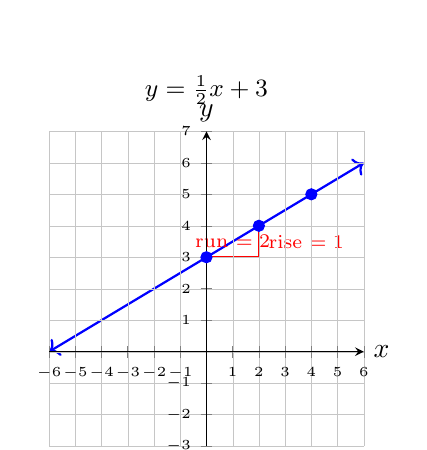
\begin{tikzpicture}\begin{axis}[gp,xmin=-6,xmax=6,ymin=-3,ymax=7,xtick={-6,...,6},ytick={-3,...,7},title={$y=\frac12x+3$}]
  \addplot[thick,blue,<->,domain=-6:6,samples=2]{x/2+3};
  \draw[red,thick] (axis cs:0,3) -- (axis cs:2,3) -- (axis cs:2,4);
  \addplot[only marks,mark=*,blue] coordinates {(0,3)(2,4)(4,5)};
  \node[red,font=\scriptsize,above] at (axis cs:1,3) {run $=2$};
  \node[red,font=\scriptsize,right] at (axis cs:2,3.5) {rise $=1$};
\end{axis}\end{tikzpicture}
\end{center}

When a linear equation is solved for $y$, the coefficient of the $x$ term is the slope and the constant term is the $y$-coordinate of the $y$-intercept.

\begin{keybox}
\textbf{Slope-Intercept Form.} The \textbf{slope-intercept form} of an equation of a line with slope $m$ and $y$-intercept $(0,b)$ is
\[y=mx+b.\]
\end{keybox}

\exbox{1} Use the graph to find the slope and $y$-intercept of the line $y=2x+1$. Compare these values to the equation $y=mx+b$. \seesol{1}
\begin{center}
\slopefig{xmin=-4,xmax=4,ymin=-4,ymax=5,xtick={-4,...,4},ytick={-4,...,5},title={$y=2x+1$}}{0}{1}{1}{3}{2*x+1}{-2.4}{2}
\end{center}

\exbox{2} Use the graph to find the slope and $y$-intercept of the line $y=\frac23x-1$. Compare these values to the equation $y=mx+b$. \seesol{2}
\begin{center}
\slopefig{xmin=-6,xmax=6,ymin=-6,ymax=6,title={$y=\frac23x-1$}}{0}{-1}{3}{1}{2*x/3-1}{-6}{6}
\end{center}

\subsection{\texorpdfstring{Identifying the Slope and $y$-Intercept from an Equation}{Identifying the Slope and y-Intercept from an Equation}}

When an equation is in slope-intercept form, the slope is the number multiplying $x$ and the $y$-intercept is $(0,b)$.

\exbox{3} Identify the slope and $y$-intercept of the line $y=-3x+5$. \seesol{3}

When an equation is not given in slope-intercept form, our first step is to solve for $y$.

\exbox{4} Identify the slope and $y$-intercept of the line $x+2y=6$. \seesol{4}

%=====================================================================
\subsection{Graphing a Line Using its Slope and Intercept}

Once we know the slope and $y$-intercept of a line from its equation, we can graph the line by plotting the $y$-intercept and then using the slope to find a second point.

\begin{keybox}
\textbf{How to graph a line using its slope and intercept.}\\
\textbf{Step 1.} Find the slope-intercept form of the equation of the line.\\
\textbf{Step 2.} Identify the slope and $y$-intercept.\\
\textbf{Step 3.} Plot the $y$-intercept.\\
\textbf{Step 4.} Use the slope formula $m=\dfrac{\text{rise}}{\text{run}}$ to identify the rise and the run.\\
\textbf{Step 5.} Starting at the $y$-intercept, count out the rise and run to mark the second point.\\
\textbf{Step 6.} Connect the points with a line.
\end{keybox}

\exbox{5} Graph the line $y=4x-2$ using its slope and $y$-intercept. \seesol{5}

\exbox{6} Graph the line $y=-x+4$ using its slope and $y$-intercept. \seesol{6}

\exbox{7} Graph the line $y=-\dfrac23x-3$ using its slope and $y$-intercept. \seesol{7}

\exbox{8} Graph the line $4x-3y=12$ using its slope and $y$-intercept. \seesol{8}

%=====================================================================
\subsection{Choosing the Most Convenient Method to Graph a Line}

We now have several methods to graph a line.

\begin{center}
\renewcommand{\arraystretch}{1.4}
\begin{tabular}{p{0.95in}|p{1.05in}|p{1.05in}|p{0.95in}}
\textbf{Point plotting} & \textbf{Slope-intercept} & \textbf{Intercepts} & \textbf{Vertical / horizontal}\\\hline
Find three points. Plot the points, make sure they line up, then draw the line. &
$y=mx+b$. Find the slope and $y$-intercept. Start at the $y$-intercept, then count the slope to get a second point. &
Find the intercepts (set $y=0$, then $x=0$) and plot the points. Draw the line. &
The equation has only one variable. $x=a$ is a vertical line, $y=b$ is a horizontal line.
\end{tabular}
\end{center}

Generally, plotting points is not the most efficient way to graph a line. Here are six equations and the method we used for each:
\begin{center}
\begin{tabular}{c l l}
\# & Equation & Method\\\hline
1 & $x=3$ & vertical line\\
2 & $y=-2$ & horizontal line\\
3 & $3x-2y=6$ & intercepts\\
4 & $-x+2y=4$ & intercepts\\
5 & $y=4x-2$ & slope-intercept\\
6 & $y=-x+4$ & slope-intercept
\end{tabular}
\end{center}

\begin{keybox}
\textbf{Strategy for choosing the most convenient method to graph a line.} Consider the form of the equation.
\begin{itemize}[itemsep=0pt]
  \item If it has only one variable, it is a vertical or horizontal line. $x=a$ is a vertical line through the $x$-axis at $a$, and $y=b$ is a horizontal line through the $y$-axis at $b$.
  \item If $y$ is isolated on one side, in the form $y=mx+b$, graph using the slope and $y$-intercept.
  \item If the equation is of the form $Ax+By=C$, find the intercepts and graph.
\end{itemize}
\end{keybox}

\exbox{9} Determine the most convenient method to graph each line. \seesol{9}
\begin{center}
$a.\ y=-6\qquad b.\ 5x-3y=15\qquad c.\ x=7\qquad d.\ y=\dfrac25x-1$
\end{center}

%=====================================================================
\pagebreak
\subsection{Examples}

\solsec{1}
Choose two points on the line, $(0,1)$ and $(1,3)$. The rise is $2$ and the run is $1$:
\[m=\frac{\text{rise}}{\text{run}}=\frac21=2.\]
The $y$-intercept is the point $(0,1)$. So $m=2$ and $y$-intercept $(0,1)$, and
\[y=\mathbf{2}x+\mathbf{1}\qquad\text{compared to}\qquad y=mx+b.\]
The slope is the same as the coefficient of $x$, and the $y$-coordinate of the $y$-intercept is the same as the constant term.

\solsec{2}
Use the points $(0,-1)$ and $(3,1)$. The rise is $2$ and the run is $3$, so $m=\frac23$. The $y$-intercept is $(0,-1)$. So
\[y=\tfrac23x+(-1)=\tfrac23x-1.\]

\solsec{3}
Compare $y=-3x+5$ to $y=mx+b$: the slope is $m=-3$ and the $y$-intercept is $(0,5)$.

\solsec{4}
This equation is not in slope-intercept form, so solve for $y$.
\begin{align*}
x+2y&=6\\
2y&=-x+6&&\text{subtract $x$ from both sides}\\
\frac{2y}2&=\frac{-x+6}2&&\text{divide both sides by $2$}\\
y&=-\frac12x+3&&\text{since }\tfrac{a+b}c=\tfrac ac+\tfrac bc
\end{align*}
The slope is $m=-\frac12$ and the $y$-intercept is $(0,3)$.

\solsec{5}
\textbf{Steps 1--2.} $y=4x-2$ is already in slope-intercept form. $m=4$ and $b=-2$, so the $y$-intercept is $(0,-2)$.\\
\textbf{Steps 3--5.} Plot $(0,-2)$. Since $m=4=\frac41$, the rise is $4$ and the run is $1$. Up $4$, right $1$ gives $(1,2)$.\\
\textbf{Step 6.} Connect the points.
\begin{center}
\slopefig{xmin=-4,xmax=4,ymin=-6,ymax=4,xtick={-4,...,4},ytick={-6,...,4},title={$y=4x-2$}}{0}{-2}{1}{2}{4*x-2}{-1}{1.5}
\end{center}

\solsec{6}
$y=-x+4$: $m=-1$ and the $y$-intercept is $(0,4)$. Plot $(0,4)$. Since $m=\frac{-1}1$, the rise is $-1$ and the run is $1$: down $1$, right $1$ gives $(1,3)$. Connect the points.
\begin{center}
\slopefig{xmin=-4,xmax=7,ymin=-2,ymax=6,xtick={-4,...,7},ytick={-2,...,6},title={$y=-x+4$}}{0}{4}{1}{3}{-x+4}{-3}{6}
\end{center}
Check: the line passes through $(4,0)$. $0\stackrel?=-4+4$, and $0=0\checkmark$.

\solsec{7}
$y=-\frac23x-3$: $m=-\frac23$ and the $y$-intercept is $(0,-3)$. Plot $(0,-3)$. The rise is $-2$ and the run is $3$: down $2$, right $3$ gives $(3,-5)$. Connect the points.
\begin{center}
\slopefig{xmin=-6,xmax=6,ymin=-7,ymax=3,xtick={-6,...,6},ytick={-7,...,3},title={$y=-\frac23x-3$}}{0}{-3}{3}{-5}{-2*x/3-3}{-5}{6}
\end{center}

\solsec{8}
First find the slope-intercept form.
\begin{align*}
4x-3y&=12\\
-3y&=-4x+12&&\text{subtract $4x$}\\
\frac{-3y}{-3}&=\frac{-4x+12}{-3}&&\text{divide by $-3$}\\
y&=\frac43x-4
\end{align*}
$m=\frac43$ and the $y$-intercept is $(0,-4)$. Plot $(0,-4)$. The rise is $4$ and the run is $3$: up $4$, right $3$ gives $(3,0)$. Connect the points.
\begin{center}
\slopefig{xmin=-4,xmax=6,ymin=-6,ymax=3,xtick={-4,...,6},ytick={-6,...,3},title={$4x-3y=12$}}{0}{-4}{3}{0}{4*x/3-4}{-1}{5}
\end{center}

\solsec{9}
$a.$ $y=-6$ has only one variable. Its graph is a horizontal line crossing the $y$-axis at $-6$.\\
$b.$ $5x-3y=15$ is of the form $Ax+By=C$. The easiest way to graph it is to find the intercepts.\\
$c.$ $x=7$ has only one variable. The graph is a vertical line crossing the $x$-axis at $7$.\\
$d.$ $y=\frac25x-1$ is in $y=mx+b$ form, so it is easiest to graph using the slope and $y$-intercept.
\clearpage
\def\chp{eqline}
\source{Elementary Algebra 2e}
\section{Finding the Equation of a Line}
The physical sciences, social sciences and the business world are full of situations that can be modeled with linear equations relating two variables. If data points appear to form a straight line, the equation of that line can be used to predict the value of one variable from the value of the other. To build such a model we need to be able to find the equation of a line. The method we use depends on what information we are given.

\subsection{\texorpdfstring{Given the Slope and $y$-Intercept}{Given the Slope and y-Intercept}}

If we know the slope and $y$-intercept, we substitute them into slope-intercept form, $y=mx+b$.

\exbox{1} Find an equation of a line with slope $-7$ and $y$-intercept $(0,-1)$. \seesol{1}

Sometimes the slope and intercept need to be read from a graph.

\exbox{2} Find the equation of the line shown. \seesol{2}
\begin{center}
\slopefig{xmin=-6,xmax=6,ymin=-6,ymax=6,title={}}{0}{-4}{3}{-2}{2*x/3-4}{-3}{6}
\end{center}

\subsection{Point-Slope Form}

What if we know the slope and a point that is not the $y$-intercept? Suppose a line has slope $m$ and contains the point $(x_1,y_1)$, and let $(x,y)$ be any other point on the line. Write the slope of the line and rewrite it:
\begin{align*}
m&=\frac{y-y_1}{x-x_1}\\
m(x-x_1)&=\frac{y-y_1}{x-x_1}(x-x_1)&&\text{multiply both sides by }x-x_1\\
m(x-x_1)&=y-y_1\\
y-y_1&=m(x-x_1)
\end{align*}

\begin{keybox}
\textbf{Point-Slope Form.} The \textbf{point-slope form} of an equation of a line with slope $m$ and containing the point $(x_1,y_1)$ is
\[y-y_1=m(x-x_1).\]
\end{keybox}

We use point-slope form to find the equation of a line when we are given the slope and one point, and then rewrite the equation in slope-intercept form, which most applications use.

\begin{keybox}
\textbf{How to find an equation of a line given the slope and a point.}\\
\textbf{Step 1.} Identify the slope.\\
\textbf{Step 2.} Identify the point.\\
\textbf{Step 3.} Substitute the values into the point-slope form $y-y_1=m(x-x_1)$.\\
\textbf{Step 4.} Write the equation in slope-intercept form.
\end{keybox}

\exbox{3} Find an equation of a line with slope $m=\dfrac25$ that contains the point $(10,3)$. Write the equation in slope-intercept form. \seesol{3}

\exbox{4} Find an equation of a line with slope $m=-\dfrac13$ that contains the point $(6,-4)$. Write the equation in slope-intercept form. \seesol{4}

\exbox{5} Find an equation of a horizontal line that contains the point $(-1,2)$. Write the equation in slope-intercept form. \seesol{5}

\subsection{Given Two Points}

When real-world data is collected, a linear model can be created from two data points. We have two options so far, slope-intercept or point-slope. Since we know two points, it makes more sense to use point-slope form. First we need the slope, which we find with the slope formula from the two points. Then we use the slope and one of the given points.

\begin{keybox}
\textbf{How to find an equation of a line given two points.}\\
\textbf{Step 1.} Find the slope using the given points, $m=\dfrac{y_2-y_1}{x_2-x_1}$.\\
\textbf{Step 2.} Choose one point.\\
\textbf{Step 3.} Substitute the values into the point-slope form $y-y_1=m(x-x_1)$.\\
\textbf{Step 4.} Write the equation in slope-intercept form.
\end{keybox}

\exbox{6} Find an equation of a line that contains the points $(5,4)$ and $(3,6)$. Write the equation in slope-intercept form. \seesol{6}

\exbox{7} Find an equation of a line that contains the points $(-3,-1)$ and $(2,-2)$. Write the equation in slope-intercept form. \seesol{7}

\exbox{8} Find an equation of a line that contains the points $(-2,4)$ and $(-2,-3)$. Write the equation in slope-intercept form. \seesol{8}

\subsection{Summary}

Which form we use depends on the information we are given.

\begin{center}
\renewcommand{\arraystretch}{1.3}
\begin{tabular}{l|l|l}
If given & Use & Form\\\hline
Slope and $y$-intercept & slope-intercept form & $y=mx+b$\\
Slope and a point & point-slope form & $y-y_1=m(x-x_1)$\\
Two points & point-slope form & $y-y_1=m(x-x_1)$
\end{tabular}
\end{center}

%=====================================================================
\pagebreak
\subsection{Examples}

\solsec{1}
We are given the slope and $y$-intercept, so substitute into $y=mx+b$.
\begin{align*}
m&=-7\\
b&=-1\quad\text{(the $y$-intercept is $(0,-1)$)}\\
y&=-7x+(-1)\\
y&=-7x-1
\end{align*}

\solsec{2}
The $y$-intercept is $(0,-4)$ and the graph passes through $(3,-2)$. Count the rise and run: the rise is $2$ and the run is $3$, so $m=\frac23$. Substitute into $y=mx+b$:
\[y=\tfrac23x-4.\]

\solsec{3}
\begin{align*}
m&=\frac25,\qquad(x_1,y_1)=(10,3)\\
y-y_1&=m(x-x_1)\\
y-3&=\frac25(x-10)\\
y-3&=\frac25x-4&&\text{distribute}\\
y&=\frac25x-1&&\text{add $3$ to both sides}
\end{align*}

\solsec{4}
\begin{align*}
m&=-\frac13,\qquad(x_1,y_1)=(6,-4)\\
y-(-4)&=-\frac13(x-6)\\
y+4&=-\frac13x+2&&\text{distribute}\\
y&=-\frac13x-2&&\text{subtract $4$ from both sides}
\end{align*}

\solsec{5}
Every horizontal line has slope $0$, so $m=0$ and $(x_1,y_1)=(-1,2)$.
\begin{align*}
y-2&=0(x-(-1))\\
y-2&=0(x+1)\\
y-2&=0\\
y&=2
\end{align*}
This is in $y$-form, but it can also be written $y=0x+2$. It is the horizontal line $y=a$ with $a=2$.

\solsec{6}
\textbf{Step 1.} Find the slope: $m=\dfrac{6-4}{3-5}=\dfrac2{-2}=-1$.\\
\textbf{Step 2.} Choose one point, $(x_1,y_1)=(5,4)$.\\
\textbf{Step 3.} Substitute into point-slope form.
\begin{align*}
y-4&=-1(x-5)\\
y-4&=-x+5&&\text{distribute}\\
y&=-x+9&&\text{add $4$ to both sides}
\end{align*}
Check: using the point $(3,6)$ gives $y-6=-1(x-3)$, so $y-6=-x+3$ and $y=-x+9$. The same equation.

\solsec{7}
Find the slope: $m=\dfrac{-2-(-1)}{2-(-3)}=\dfrac{-1}5=-\dfrac15$.\\
Choose the point $(2,-2)$.
\begin{align*}
y-(-2)&=-\frac15(x-2)\\
y+2&=-\frac15x+\frac25\\
y&=-\frac15x+\frac25-\frac{10}5\\
y&=-\frac15x-\frac85
\end{align*}

\solsec{8}
Find the slope: $m=\dfrac{-3-4}{-2-(-2)}=\dfrac{-7}0$, which is \textbf{undefined}. This tells us the line is vertical. Both points have an $x$-coordinate of $-2$, so the equation of the line is $x=-2$. Since there is no $y$, we cannot write it in slope-intercept form. (Sketching the two points confirms that this is a vertical line.)
\part{Systems of Equations}

\clearpage
\def\chp{systems}
\source{Elementary Algebra}
\section{Solving Systems of Equations}
\subsection{Is an Ordered Pair a Solution?}

\begin{keybox}
When two or more linear equations are grouped together, they form a \textbf{system of linear equations}.
\end{keybox}

We focus on systems of two linear equations in two unknowns. We use a brace to show the equations are grouped together. For example:
\[\begin{cases}2x+y=7\\x-2y=6\end{cases}\]

A linear equation in two variables, like $2x+y=7$, has infinitely many solutions. Its graph is a line, and every point on the line is a solution to the equation, and every solution is a point on the line. To solve a system we find the ordered pairs $(x,y)$ that make \textbf{both} equations true.

\begin{keybox}
\textbf{Solutions of a system of equations} are the values of the variables that make \textbf{all} the equations true. A solution of a system of two linear equations is represented by an ordered pair $(x,y)$.
\end{keybox}

To determine if an ordered pair is a solution, substitute the values into \textbf{both} equations. If the pair makes both equations true, it is a solution of the system. Consider the system
\[\begin{cases}3x-y=7\\x-2y=4\end{cases}\]
Is $(2,-1)$ a solution? Substitute $x=2$ and $y=-1$:
\[3(2)-(-1)=6+1=7\ \checkmark\qquad\qquad2-2(-1)=2+2=4\ \checkmark\]
Both are true, so $(2,-1)$ is a solution. Is $(3,2)$ a solution? Substitute $x=3$ and $y=2$:
\[3(3)-2=7\ \checkmark\qquad\qquad3-2(2)=-1\neq4\ \times\]
It made one equation true but the other false, so $(3,2)$ is \textbf{not} a solution.

\exbox{1} Determine whether the ordered pair is a solution to the system
\[\begin{cases}x-y=-1\\2x-y=-5\end{cases}\]
$a.\ (-2,-1)\qquad\qquad b.\ (-4,-3)$ \seesol{1}

\subsection{Types of Systems}

It is possible for a system to have no solution.

\begin{keybox}
A \textbf{consistent} system of equations is a system with at least one solution.\\
An \textbf{inconsistent} system of equations is a system with no solution.
\end{keybox}

We also describe the equations in a system as independent or dependent.

\begin{keybox}
Two equations are \textbf{independent} if they have different solutions.\\
Two equations are \textbf{dependent} if all the solutions of one equation are also solutions of the other equation.
\end{keybox}

%=====================================================================
\subsection{Solving Systems of Equations by Substitution}

Consider the system $\begin{cases}2x+y=7\\x-2y=6\end{cases}$. We first solve one of the equations for either $x$ or $y$, choosing whichever keeps the work easy. Then we substitute that expression into the \emph{other} equation. The result is an equation with just one variable, which we know how to solve! After we find one variable, we substitute that value into one of the original equations and solve for the other variable. Finally we check that our solution makes both equations true.

\begin{keybox}
\textbf{How to solve a system of equations by substitution.}\\
\textbf{Step 1.} Solve one of the equations for either variable.\\
\textbf{Step 2.} Substitute the expression from Step 1 into the other equation.\\
\textbf{Step 3.} Solve the resulting equation.\\
\textbf{Step 4.} Substitute the solution from Step 3 into one of the original equations to find the other variable.\\
\textbf{Step 5.} Write the solution as an ordered pair.\\
\textbf{Step 6.} Check that the ordered pair is a solution to \textbf{both} original equations.
\end{keybox}

\exbox{2} Solve by substitution. \seesol{2}
\[\begin{cases}2x+y=7\\x-2y=6\end{cases}\]

If one of the equations is already solved for a variable, Step 1 is already done.

\exbox{3} Solve by substitution. \seesol{3}
\[\begin{cases}x+y=-1\\y=x+5\end{cases}\]

In Example 4 it is easiest to solve for $y$ in the first equation, because it has a coefficient of $1$. In Example 5 it is easiest to solve for $x$.

\exbox{4} Solve by substitution. \seesol{4}
\[\begin{cases}3x+y=5\\2x+4y=-10\end{cases}\]

\exbox{5} Solve by substitution. \seesol{5}
\[\begin{cases}x-2y=-2\\3x+2y=34\end{cases}\]

When both equations are already solved for the same variable, it is easy to substitute.

\exbox{6} Solve by substitution. \seesol{6}
\[\begin{cases}y=\frac12x\\y=-2x+5\end{cases}\]

Be very careful with the signs in the next example.

\exbox{7} Solve by substitution. \seesol{7}
\[\begin{cases}4x+2y=4\\6x-y=8\end{cases}\]

\exbox{8} Solve by substitution. \seesol{8}
\[\begin{cases}4x-3y=6\\15y-20x=-30\end{cases}\]

\exbox{9} Solve by substitution. \seesol{9}
\[\begin{cases}5x-2y=-10\\y=\frac52x\end{cases}\]

\begin{keybox}
If solving leaves a \textbf{true} statement like $0=0$, the system is \textbf{consistent} and the equations are \textbf{dependent}. There are infinitely many solutions.\\
If solving leaves a \textbf{false} statement like $0=-10$, the system is \textbf{inconsistent}. There is no solution.
\end{keybox}

%=====================================================================
\subsection{Solving Systems of Equations by Elimination}

Substitution works well when we can easily solve one equation for a variable without too many fractions. The second method, \textbf{elimination}, is based on the Addition Property of Equality: when you add the same quantity to both sides of an equation you still have equality. We extend it to say that adding equal quantities to both sides keeps the equation equal.

\begin{center}
For any expressions $a,b,c,d$: if $a=b$ and $c=d$ then $a+c=b+d$.
\end{center}

To solve a system by elimination, start with both equations in standard form, $Ax+By=C$. Then decide which variable is easiest to eliminate by making its coefficients \textbf{opposites}, so that adding the equations eliminates that variable. For example,
\[
\begin{array}{r}3x+y=5\\+\ \ 2x-y=0\\\hline5x\phantom{{}+y}=5\end{array}
\]
The $y$'s add to zero and we have one equation with one variable. Let's try
\[\begin{cases}x+4y=2\\2x+5y=-2\end{cases}\]
We don't see a variable we can eliminate by adding yet. But if we multiply the first equation by $-2$ (every term!), the coefficients of $x$ are opposites:
\[\begin{array}{r}-2x-8y=-4\\+\ \ 2x+5y=-2\\\hline-3y=-6\end{array}\]
so $y=2$. Substituting into $x+4y=2$ gives $x+8=2$, so $x=-6$. The solution is $(-6,2)$. Check: $2(-6)+5(2)=-12+10=-2\checkmark$.

\begin{keybox}
\textbf{How to solve a system of equations by elimination.}\\
\textbf{Step 1.} Write both equations in standard form. If any coefficients are fractions, clear them.\\
\textbf{Step 2.} Make the coefficients of one variable opposites. Decide which variable you will eliminate, then multiply one or both equations so that the coefficients of that variable are opposites.\\
\textbf{Step 3.} Add the equations resulting from Step 2 to eliminate one variable.\\
\textbf{Step 4.} Solve for the remaining variable.\\
\textbf{Step 5.} Substitute the solution from Step 4 into one of the original equations. Then solve for the other variable.\\
\textbf{Step 6.} Write the solution as an ordered pair.\\
\textbf{Step 7.} Check that the ordered pair is a solution to \textbf{both} original equations.
\end{keybox}

Sometimes we must multiply \textbf{both} equations by constants. For
\[\begin{cases}4x-3y=10\\3x+5y=-7\end{cases}\]
we cannot get opposite coefficients by multiplying one equation by a constant unless we use fractions. Instead multiply the first equation by $3$ and the second by $-4$ so that the $x$ terms become $12x$ and $-12x$:
\[\begin{array}{r}12x-9y=30\\-12x-20y=28\\\hline-29y=58\end{array}\]
so $y=-2$, then $4x-3(-2)=10$ gives $4x=4$ and $x=1$. The solution is $(1,-2)$. Check: $3(1)+5(-2)=3-10=-7\checkmark$.

\exbox{10} Solve by elimination (the same system we solved by substitution). \seesol{10}
\[\begin{cases}2x+y=7\\x-2y=6\end{cases}\]

\exbox{11} Solve by elimination. \seesol{11}
\[\begin{cases}x+y=10\\x-y=12\end{cases}\]

\exbox{12} Solve by elimination. \seesol{12}
\[\begin{cases}3x-2y=-2\\5x-6y=10\end{cases}\]

\exbox{13} Solve by elimination. \seesol{13}
\[\begin{cases}4x-3y=9\\7x+2y=-6\end{cases}\]

When the system contains fractions, first clear them by multiplying each equation by its LCD.

\exbox{14} Solve by elimination. \seesol{14}
\[\begin{cases}x+\frac12y=6\\\frac32x+\frac23y=\frac{17}2\end{cases}\]

\exbox{15} Solve by elimination. \seesol{15}
\[\begin{cases}3x+4y=12\\y=3-\frac34x\end{cases}\]

\exbox{16} Solve by elimination. \seesol{16}
\[\begin{cases}-6x+15y=10\\2x-5y=-5\end{cases}\]

%=====================================================================
\pagebreak
\subsection{Examples}

\solsec{1}
$a.$ Substitute $x=-2$, $y=-1$:
\[-2-(-1)=-1\ \checkmark\qquad\qquad2(-2)-(-1)=-4+1=-3\neq-5\ \times\]
$(-2,-1)$ is \textbf{not} a solution.\\
$b.$ Substitute $x=-4$, $y=-3$:
\[-4-(-3)=-1\ \checkmark\qquad\qquad2(-4)-(-3)=-8+3=-5\ \checkmark\]
$(-4,-3)$ \textbf{is} a solution.

\solsec{2}
\begin{align*}
\text{Step 1: }&\text{solve the first equation for }y:\quad 2x+y=7\ \to\ y=7-2x\\
\text{Step 2: }&\text{substitute into the second equation:}\quad x-2(7-2x)=6\\
\text{Step 3: }&\text{solve for }x:\quad x-14+4x=6\ \to\ 5x=20\ \to\ x=4\\
\text{Step 4: }&\text{substitute into }2x+y=7:\quad 2(4)+y=7\ \to\ y=-1\\
\text{Step 5: }&\text{ordered pair:}\quad (4,-1)
\end{align*}
Step 6, check: $2(4)+(-1)=7\checkmark$ and $4-2(-1)=6\checkmark$. The solution is $(4,-1)$.

\solsec{3}
The second equation is already solved for $y$. Substitute $x+5$ for $y$ in the first equation.
\begin{align*}
x+(x+5)&=-1\\
2x+5&=-1\\
2x&=-6\\
x&=-3
\end{align*}
Substitute into $y=x+5$: $y=-3+5=2$. The solution is $(-3,2)$.\\
Check: $-3+2=-1\checkmark$ and $2=-3+5\checkmark$.

\solsec{4}
Solve the first equation for $y$: $y=-3x+5$. Substitute into the second equation.
\begin{align*}
2x+4(-3x+5)&=-10\\
2x-12x+20&=-10\\
-10x&=-30\\
x&=3
\end{align*}
Substitute $x=3$ into $3x+y=5$: $9+y=5$, so $y=-4$. The solution is $(3,-4)$.

\solsec{5}
Solve the first equation for $x$: $x=2y-2$. Substitute into the second equation.
\begin{align*}
3(2y-2)+2y&=34\\
6y-6+2y&=34\\
8y&=40\\
y&=5
\end{align*}
Substitute $y=5$ into $x-2y=-2$: $x-10=-2$, so $x=8$. The solution is $(8,5)$.

\solsec{6}
Both equations are solved for $y$, so substitute $\frac12x$ for $y$ in the second equation.
\begin{align*}
\tfrac12x&=-2x+5\\
2\left(\tfrac12x\right)&=2(-2x+5)&&\text{clear the fraction}\\
x&=-4x+10\\
5x&=10\\
x&=2
\end{align*}
Substitute into $y=\frac12x$: $y=\frac12\cdot2=1$. The solution is $(2,1)$.

\solsec{7}
Solve the first equation for $y$: $2y=-4x+4$, so $y=-2x+2$. Substitute into the second equation.
\begin{align*}
6x-(-2x+2)&=8\\
6x+2x-2&=8\\
8x&=10\\
x&=\frac54
\end{align*}
Substitute into $4x+2y=4$: $4\left(\frac54\right)+2y=4$, so $5+2y=4$, $2y=-1$ and $y=-\frac12$. The solution is $\left(\frac54,-\frac12\right)$.

\solsec{8}
Solve the first equation for $x$: $4x=3y+6$, so $x=\frac34y+\frac32$. Substitute into the second equation.
\begin{align*}
15y-20\left(\tfrac34y+\tfrac32\right)&=-30\\
15y-15y-30&=-30\\
-30&=-30\\
0&=0
\end{align*}
Since $0=0$ is a true statement, the system is consistent and the equations are dependent. The system has \textbf{infinitely many solutions}.

\solsec{9}
Substitute $\frac52x$ for $y$ in the first equation.
\begin{align*}
5x-2\left(\tfrac52x\right)&=-10\\
5x-5x&=-10\\
0&=-10
\end{align*}
Since $0=-10$ is a false statement, the equations are inconsistent. The system has \textbf{no solution}.

\solsec{10}
\textbf{Steps 1--2.} Both equations are in standard form with no fractions. Multiply the first equation by $2$ so the $y$ coefficients are opposites:
\[2(2x+y)=2(7)\ \to\ 4x+2y=14.\]
\textbf{Step 3.} Add:
\[\begin{array}{r}4x+2y=14\\x-2y=6\\\hline5x\phantom{{}+2y}=20\end{array}\]
\textbf{Step 4.} $x=4$.\\
\textbf{Step 5.} Substitute into $x-2y=6$: $4-2y=6$, so $-2y=2$ and $y=-1$.\\
\textbf{Steps 6--7.} The solution is $(4,-1)$. Check: $2(4)+(-1)=7\checkmark$ and $4-2(-1)=6\checkmark$. (The same answer as by substitution.)

\solsec{11}
The coefficients of $y$ are already opposites. Add the equations:
\[\begin{array}{r}x+y=10\\x-y=12\\\hline2x\phantom{{}+y}=22\end{array}\]
So $x=11$. Substitute into $x+y=10$: $11+y=10$, so $y=-1$. The solution is $(11,-1)$.\\
Check: $11+(-1)=10\checkmark$ and $11-(-1)=12\checkmark$.

\solsec{12}
Multiply the first equation by $-3$ to make the $y$ coefficients opposites:
\[-3(3x-2y)=-3(-2)\ \to\ -9x+6y=6.\]
Add to the second equation:
\[\begin{array}{r}-9x+6y=6\\5x-6y=10\\\hline-4x\phantom{{}+6y}=16\end{array}\]
So $x=-4$. Substitute into $3x-2y=-2$: $-12-2y=-2$, so $-2y=10$ and $y=-5$. The solution is $(-4,-5)$.\\
Check: $3(-4)-2(-5)=-12+10=-2\checkmark$ and $5(-4)-6(-5)=-20+30=10\checkmark$.

\solsec{13}
We multiply both equations by constants. To make the $y$ coefficients opposites, multiply the first equation by $2$ and the second by $3$:
\[\begin{array}{r}8x-6y=18\\21x+6y=-18\\\hline29x\phantom{{}+6y}=0\end{array}\]
So $x=0$. Substitute into $7x+2y=-6$: $2y=-6$, so $y=-3$. The solution is $(0,-3)$.\\
Check: $4(0)-3(-3)=9\checkmark$ and $7(0)+2(-3)=-6\checkmark$.

\solsec{14}
Clear the fractions: multiply the first equation by $2$ and the second by $6$.
\begin{align*}
2\left(x+\tfrac12y\right)&=2(6)&\to\quad2x+y&=12\\
6\left(\tfrac32x+\tfrac23y\right)&=6\left(\tfrac{17}2\right)&\to\quad9x+4y&=51
\end{align*}
Eliminate $y$ by multiplying the top equation by $-4$:
\[\begin{array}{r}-8x-4y=-48\\9x+4y=51\\\hline x\phantom{{}+4y}=3\end{array}\]
Substitute $x=3$ into $x+\frac12y=6$: $3+\frac12y=6$, so $\frac12y=3$ and $y=6$. The solution is $(3,6)$.\\
Check: $3+\frac12(6)=6\checkmark$ and $\frac32(3)+\frac23(6)=\frac92+4=\frac{17}2\checkmark$.

\solsec{15}
Write the second equation in standard form: $\frac34x+y=3$. Clear the fractions by multiplying by $4$: $3x+4y=12$. Now the system is
\[\begin{cases}3x+4y=12\\3x+4y=12\end{cases}\]
To eliminate a variable, multiply the second equation by $-1$ and add:
\[\begin{array}{r}3x+4y=12\\-3x-4y=-12\\\hline0=0\end{array}\]
This is a true statement. The equations are consistent but dependent. The system has \textbf{infinitely many solutions}.

\solsec{16}
The equations are in standard form. Multiply the second equation by $3$ to eliminate a variable:
\[\begin{array}{r}-6x+15y=10\\6x-15y=-15\\\hline0=-5\end{array}\]
This statement is false. The equations are inconsistent. The system has \textbf{no solution}.
\end{document}
